\documentclass[11pt]{aghdpl}
% \documentclass[en,11pt]{aghdpl}  % praca w języku angielskim

% Lista wszystkich języków stanowiących języki pozycji bibliograficznych użytych w pracy.
% (Zgodnie z zasadami tworzenia bibliografii każda pozycja powinna zostać utworzona zgodnie z zasadami języka, w którym dana publikacja została napisana.)
\usepackage[english,polish]{babel}

% Użyj polskiego łamania wyrazów (zamiast domyślnego angielskiego).
\usepackage{polski}

\usepackage[utf8]{inputenc}

% dodatkowe pakiety

\usepackage{mathtools}
\usepackage{amsfonts}
\usepackage{amsmath}
\usepackage{amsthm}

% --- < bibliografia > ---

\usepackage[
style=numeric,
sorting=none,
%
% Zastosuj styl wpisu bibliograficznego właściwy językowi publikacji.
language=autobib,
autolang=other,
% Zapisuj datę dostępu do strony WWW w formacie RRRR-MM-DD.
urldate=iso8601,
% Nie dodawaj numerów stron, na których występuje cytowanie.
backref=false,
% Podawaj ISBN.
isbn=true,
% Nie podawaj URL-i, o ile nie jest to konieczne.
url=false,
%
% Ustawienia związane z polskimi normami dla bibliografii.
maxbibnames=3,
% Jeżeli używamy BibTeXa:
backend=biber
]{biblatex}

\usepackage{csquotes}
% Ponieważ `csquotes` nie posiada polskiego stylu, można skorzystać z mocno zbliżonego stylu chorwackiego.
\DeclareQuoteAlias{croatian}{polish}

\addbibresource{bibliografia.bib}

% Nie wyświetlaj wybranych pól.
%\AtEveryBibitem{\clearfield{note}}


% ------------------------
% --- < listingi > ---

% Użyj czcionki kroju Courier.
\usepackage{courier}

\usepackage{listings}
\lstloadlanguages{TeX}

\lstset{
	literate={ą}{{\k{a}}}1
           {ć}{{\'c}}1
           {ę}{{\k{e}}}1
           {ó}{{\'o}}1
           {ń}{{\'n}}1
           {ł}{{\l{}}}1
           {ś}{{\'s}}1
           {ź}{{\'z}}1
           {ż}{{\.z}}1
           {Ą}{{\k{A}}}1
           {Ć}{{\'C}}1
           {Ę}{{\k{E}}}1
           {Ó}{{\'O}}1
           {Ń}{{\'N}}1
           {Ł}{{\L{}}}1
           {Ś}{{\'S}}1
           {Ź}{{\'Z}}1
           {Ż}{{\.Z}}1,
	basicstyle=\footnotesize\ttfamily,
}

% ------------------------

\AtBeginDocument{
	\renewcommand{\tablename}{Tabela}
	\renewcommand{\figurename}{Rys.}
}

% ------------------------
% --- < tabele > ---

\usepackage{array}
\usepackage{tabularx}
\usepackage{multirow}
\usepackage{booktabs}
\usepackage{makecell}
\usepackage[flushleft]{threeparttable}

% defines the X column to use m (\parbox[c]) instead of p (`parbox[t]`)
\newcolumntype{C}[1]{>{\hsize=#1\hsize\centering\arraybackslash}X}


%---------------------------------------------------------------------------

\author{Bartłomiej Łazarczyk}
\shortauthor{B. Łazarczyk}

%\titlePL{Przygotowanie bardzo długiej i pasjonującej pracy dyplomowej w~systemie~\LaTeX}
%\titleEN{Preparation of a very long and fascinating bachelor or master thesis in \LaTeX}

\titlePL{Inteligentna platforma służąca do komunikacji oraz wymiany informacji pomiędzy autorami projektów wykorzystująca algorytmy uczenia maszynowego}
%\titleEN{Thesis in \LaTeX}


\shorttitlePL{Platforma służąca do komunikacji oraz wymiany informacji pomiędzy autorami projektów} % skrócona wersja tytułu jeśli jest bardzo długi
%\shorttitleEN{Preparation of a long and fascinating thesis in \LaTeX}

\thesistype{Praca dyplomowa inżynierska}
%\thesistype{Master of Science Thesis}

\supervisor{dr hab. inż. Jarosław Wąs, prof. AGH}
%\supervisor{Marcin Szpyrka PhD, DSc}

\degreeprogramme{Informatyka}
%\degreeprogramme{Computer Science}

\date{2019}

\department{Katedra Informatyki Stosowanej}
%\department{Department of Applied Computer Science}

\faculty{Wydział Elektrotechniki, Automatyki,\protect\\[-1mm] Informatyki i Inżynierii Biomedycznej}
%\faculty{Faculty of Electrical Engineering, Automatics, Computer Science and Biomedical Engineering}

\acknowledgements{Serdecznie dziękuję \dots }


\setlength{\cftsecnumwidth}{10mm}

%---------------------------------------------------------------------------
\setcounter{secnumdepth}{4}
\brokenpenalty=10000\relax

\begin{document}

\titlepages

% Ponowne zdefiniowanie stylu `plain`, aby usunąć numer strony z pierwszej strony spisu treści i poszczególnych rozdziałów.
\fancypagestyle{plain}
{
	% Usuń nagłówek i stopkę
	\fancyhf{}
	% Usuń linie.
	\renewcommand{\headrulewidth}{0pt}
	\renewcommand{\footrulewidth}{0pt}
}

\setcounter{tocdepth}{2}
\tableofcontents
\clearpage



\chapter{Wstęp}
\label{cha:wstep}

\section{Cel pracy}
\label{sec:celPracy}

Celem pracy jest zaprojektowanie aplikacji internetowej o nazwie \mbox{\textit{ProjectSHARE}}, która ma na celu wspomagać oraz uprościć wymianę informacji między zespołami zaangażowanymi w tworzenie
projektów o podobnej tematyce. Aplikacja ma postać platformy, dzięki której użytkownik
może: stworzyć projekt prywatny bądź publiczny, wyszukać inicjatywy tworzone przez
innych użytkowników oraz dołączyć do istniejącego już projektu. Dodatkowo platforma zawiera system rekomendacji projektów uwzględniający preferencje użytkownika.

\section{Opis problemu}
\label{sec:opisProblemu}
Tworząc różnego rodzaju projekty takie jak np. praca inżynierska, projekt uczelniany, 
projekt tworzony dla koła naukowego czy zaawansowany produkt biznesowy, często pojawiają się
problemy, które blokują dalszą pracę. Twórcy sięgają wtedy po źródła dostępne w
internecie, jednak nie zawsze są one w stanie im pomóc bądź wiarygodność ich autorów jest
nieznana. W danej sytuacji jednym z najbardziej pomocnych rozwiązań jest kontakt z osobą
która ma większe doświadczenie oraz miała styczność z implementacją podobnej
funkcjonalności w celu konsultacji problemu. Możliwość takiego kontaktu zapewnia kilka
popularnych repozytorium takich jak np. GitHub, jednak mają one kilka wad: zawierają głównie
projekty z branży IT, brakuje możliwości łatwego wyszukania projektów oraz często
wymagają udostępnienia całej implementacji, ponieważ stworzenie prywatnego
repozytorium wymaga opłaty. Można również dodać, że firmy produkujące oprogramowanie
biznesowe mają swoje własne repozytoria, więc wyszukanie projektu oraz kontakt z
doświadczonym pracownikiem jest trudny. 


Po przeanalizowaniu wyżej wymienionych scenariuszy powstał pomysł na stworzenie aplikacji         
\mbox{ProjectSHARE}, która będzie uwzględniać każdy z nich w fazie projektowania oraz rozwiąże wynikające z nich problemy użytkownika systemu skierowanego do autorów projektów.

\newpage

\section{Zakres pracy}
\label{sec:zakresPracy}

W ramach pracy inżynierskiej wykonano:
\begin{itemize}
	\item Przegląd literatury dotyczącej metodologii wytwarzania oprogramowania oraz stosowanych w ich obrębie technik
	\item Przegląd literatury dotyczącej technologii potrzebnych do stworzenia aplikacji internetowej oraz zasady działania każdej z nich
	\item Przegląd literatury dotyczącej algorytmów stosowanych w systemach rekomendacji oraz wybór odpowiedniego algorytmu bazując na ustalonych założeniach systemu	
	\item Projekt architektury aplikacji, interfejsu użytkownika oraz modelu bazy danych
	\item Implementację elementów tworzonej platformy określonych w wymaganiach
	\item Implementację wybranego algorytmu uczenia maszynowego dotyczącego systemu rekomendacji

	
\end{itemize}
\chapter{Wprowadzenie teoretyczne}
\label{cha:wprowadzenieTeoretyczne}

\section{Dobór odpowiedniej metodologii}
\label{sec:doborMetodologi}

Tworząc aplikację internetową pierwszym i prawdopodobnie najważniejszym krokiem
jest dobranie metodologii wytwarzania oprogramowania oraz ogólnych praktyk, które
należy stosować. Obecnie dwa najpopularniejsze podejścia do zarządzania projektem
praktykowane w przedsiębiorstwach to model kaskadowy (ang. waterfall) oraz model
zwinny (ang. agile).

\subsection{Model kaskadowy}
\label{subsec:modelKaskadowy}
Podejście waterfall jest klasycznym systemem używanym w wielu branżach,
polegającym na wyszczególnieniu konkretnych faz projektowych, następujących kolejno po sobie. W
przypadku projektów informatycznych fazy te są następujące: faza koncepcyjna, rozpoczęcie,
analiza, projektowanie, budowa, testy, produkcja/wdrożenie oraz obsługa. Główne
założenia tego modelu to: szczegółowy plan, sekwencyjna realizacja zadań, rygorystyczne
przestrzeganie terminów oraz konsekwentne prowadzenie dokumentacji. Zalety tego
podejścia to między innymi określenie bardzo szczegółowych wymagań klienta na początku
całego procesu, jasno określone rezultaty oraz zmniejszone prawdopodobieństwo
nieporozumień wewnątrz zespołu, bądź na linii klient-realizator. Model ten posiada jednak
kilka wad takich jak brak możliwości powrotu do wcześniejszej fazy oraz 
modyfikacji wymagań klienta podczas rozwoju aplikacji, możliwość przeprowadzenia
fazy testowania dopiero pod koniec procesu, co wiąże się z dodatkowymi kosztami na wielu
poziomach. Na podstawie wyżej wymienionych zalet oraz wad można wysnuć wnioski, że
model ten nadaje się do realizacji projektów o jasno określonych wymaganiach, gdzie
dokładność jest ważniejsza niż szybkość wykonania. Niestety obecnie w obszarze tworzenia
oprogramowania coraz częściej pojawiają się dynamicznie zmieniające się wymagania klientów, dużą konkurencje, niestabilny rynek, brak jednolitych standardów i regulacji przez
co model ten wydaje się przestarzały, ryzykowny i nieopłacalny.
\subsection{Model zwinny}
\label{subsec:modelZwinny}
W odpowiedzi na potrzeby zespołów programistów w 2001 roku powstał koncept
podejścia zwinnego. Jego założenia były zupełnie inne niż w przypadku podejścia
kaskadowego. Indywidualności oraz interakcje zamiast procesów i narzędzi, działające
oprogramowanie zamiast obszernej dokumentacji, bezpośrednia i stała współpraca z klientem
zamiast negocjacji kontraktu, odpowiedź na zmienne wymagania zamiast podążania za z góry
wytyczonym planem. Dziś podejście agile nie jest uważane za konkretną metodologię,
a raczej za zbiór pomysłów, które można stosować w wielu kombinacjach, dostosowanych do
potrzeb projektu oraz zespołu.


Nowoczesne, zwinne podejście opiera się na pięciu zasadach. Pierwszą z nich jest
jasno zdefiniowana rola menadżera, dewelopera, klienta oraz zespołu. Zespół jako całość ma
obowiązek podziału zadań do wykonania oraz przydzielania ich do poszczególnych członków zespołu. Rola
klienta natomiast nie sprowadza się do bycia pasywnym, lecz staje się on aktywnym
uczestnikiem procesu wytwarzania oprogramowania. Drugą zasadą jest odrzucenie wymagań
oraz fazy projektowania na początku procesu, ponieważ klient nie może w 100 procentach wiedzieć czego dokładnie chce i
nie jest w stanie tego określić na takim etapie. Zamiast tego stosowana jest ciągła współpraca
z klientem, który dynamicznie ustala swoje wymagania co do produktu. Następną zasadą jest
stosowanie iteracji. Na początku każdej iteracji określane są jej wymagania oraz lista
funkcjonalności do zaimplementowania. Każda iteracja trwa małą, określoną ilość czasu oraz
zakłada brak dodawania wymagań podczas tego okresu. Krótki czas zmniejsza również
koszty związane z implementacją funkcjonalności, które mogą stać się nieaktualne pod koniec
iteracji. Kolejnym dogmatem jest ograniczenie niepotrzebnej funkcjonalności. Oznacza to, że
każda funkcjonalność ma określoną wartość biznesową, dzięki czemu zespół nie
implementuje czegoś, co nie będzie nigdy użyte w końcowym produkcie. Dodatkowo ustala
się potencjalny czas wykonania danej funkcjonalności w celu lepszego przydzielenia zadań na
iterację. Ostatnia zasada skupia się na jakości wytwarzanego oprogramowania. W metodach
zwinnych jest ona uzyskiwana poprzez ciągłe testowanie na przestrzeni całego procesu
tworzenia produktu. Aby funkcjonalność została zaakceptowana i wdrożona na produkcję
musi przejść wszystkie testy.

\section{Dobór odpowiednich technik wytwarzania oprogramowania}
\label{sec:doborTechnikWytwarzania}

Wydawało by się, że metodologia zwinna nadaje się do każdego projektu
informatycznego, jednak praktyka na przestrzeni wielu lat pokazała, że są one często
nadinterpretowane, bądź potencjalna wartość dodana stosowanej praktyki jest mocno
zawyżona. W rzetelnej analizie najpopularniejszych technik zwinnych nieocenioną pomocą
okazały się wiadomości zawarte w książce „Agile!”, której autorem jest Bertrand Meyer oraz
badania opisane w książce „Test-Driven Development. An Empirical Evaluation of Agile
Practice” Lecha Madeyskiego. Pierwsza pozycja odnosi się do tez głoszonych przez
autorytety w dziedzinie inżynierii oprogramowania dotyczących metodyki zwinnej oraz ocenia powszechnie stosowane
metody, opierając się na wieloletnim doświadczeniu zdobytym przez programistów. Druga
opisuje badania przeprowadzone na studentach Politechniki Wrocławskiej, które dotyczą
dwóch najbardziej popularnych praktyk czyli Pair Programming oraz Test-Driven
Development. Eksperyment miał pokazać wpływ wyżej wymienionych praktyk m.in. na testy
akceptacyjne, stopień powiązania ze sobą nowo utworzonych klas, pokrycie kodu testami
jednostkowymi oraz liczbę defektów. Po zapoznaniu się z obiema pozycjami można wyróżnić
kilka technik, które wydają się być najbardziej odpowiednie dla realizowanego projektu.

\subsection{Krótkie iteracje}
\label{subsec:krótkieIteracje}

Wspomniane wcześniej krótkie iteracje oraz wiążące się z nimi zamknięcie się na
jakiekolwiek dodawanie nowych funkcjonalności w ich obrębie, brak opóźnień pomimo nie
wykonania wszystkich zadań oraz skupienie się na dostarczeniu działającego oprogramowania na koniec każdej z nich są prawdopodobnie najważniejszymi praktykami
wprowadzonymi przez podejście zwinne. Wielu specjalistów docenia je ze względu na
częste punkty kontrolne podczas procesu produkcji oprogramowania oraz możliwość
otrzymania niemal natychmiastowej informacji zwrotnej od klienta. Brak opóźnień w iteracji
wraz z zamknięciem się na zmianę wymagań sprawiają, że nic nie zakłóca pracy i programista
jest w stanie bardziej skupić się na konkretnym zadaniu. Dodatkową zaletą jest dłuższy okres
określenia wartości biznesowej danego pomysłu przez klienta, dzięki czemu może
lepiej sprecyzować swoje zapotrzebowania. W przypadku projektu, w którym wymagania będą
się zmieniały bardzo dynamicznie najlepszym wyborem jest 14 dniowy okres jednej iteracji,
ponieważ gwarantuje to możliwość modyfikacji założeń lub wymagań w bardzo krótkim
czasie, co wydaje się kluczowe podczas tak ograniczonego czasu na wykonanie projektu.

\subsection{Faza projektowania i ustalenia wymagań}
\label{subsec:fazaProjektowania}

Następną, mocno kontrowersyjną praktyką jest odrzucenie wymagań oraz fazy
projektowania na początku procesu. Nie można zaprzeczyć, że określenie wszystkich
potrzebnych wymagań na początku jest niemożliwe. Wraz z postępami architektura systemu
również będzie wielokrotnie zmieniana, dlatego teoretycznie z biznesowego punktu widzenia
faza projektowania jest nieopłacalna. Z drugiej strony wnikliwe przestudiowanie problemu
przed próbą rozwiązania go znacząco poprawia początkową pracę zespołu, dlatego
doświadczeni inżynierowie nie pomijają tego kroku. Jednak w przeciwieństwie do założeń
modelu kaskadowego, wymagania ustalone podczas fazy projektowania powinny być
traktowane jak każdy inny artefakt, czyli ulegać zmianie wraz z postępem prac.
Dodatkowo jakiekolwiek wymagania nie powinny się składać tylko i wyłącznie ze
scenariuszy użytkownika systemu, ponieważ nie pokazują one abstrakcji różnych
komponentów. Opierając się tylko na nich programista nie jest w stanie stworzyć funkcjonalności
łatwych do zaadaptowania w nowych przypadkach. Wymienione scenariusze powinny być
uzupełnieniem wymagań, potwierdzać ich kompletność. Biorąc pod uwagę wszystkie
argumenty za i przeciw można wysnuć wniosek, że przeprowadzenie fazy projektowania i
ustalenia wstępnych wymagań w celu zaprojektowania ogólnej architektury projektu oraz
zdefiniowania funkcjonalności aplikacji jest krokiem koniecznym. Jednak zgodnie z
podejściem zwinnym ustalenia te będą się zmieniały.

\subsection{Planning poker}
\label{subsec:planningPoker}
Jest to technika wywodząca się z podejścia \textit{Scrum}, mająca za zadanie ułatwić proces estymacji kosztu wyprodukowania danej funkcjonalności. Polega ona na przydzieleniu poszczególnym historyjką użytkownika punktów o nazwie \textit{Story points}, które mają symbolizować koszt związany z daną historyjką. W ramach tej techniki muszą zostać spełnione poniższe założenia\cite{AGI01}:
\begin{itemize}
\item poleganie na kolektywnym osądzie całego zespołu
\item przeprowadzanie iteracji do momentu uzyskania zgody wszystkich członków zespołu
\item unikanie niepotrzebnego przestoju wynikającego z małych różnic, dzięki ustaleniu ciągu liczb, którymi można określić \textit{Story points}
\end{itemize}

Najczęściej wybieranym ciągiem liczb jest ciąg Fibonacciego, czyli wartości \mbox{0, 1, 2, 3, 5, 8, 13, 21, ...} . Jeżeli estymacja symbolizuje ilość dni, które dana osoba musi przeznaczyć na wytworzenie danej funkcjonalności, wtedy często dodaje się wartość 0.5, która oznacza mniej niż jeden dzień. Zaletą tego podejścia jest uniknięcie niepotrzebnych dyskusji w zespole, które wynikałyby z nieznaczących różnic w wartościach np. między 11 a 12. Dodatkowo wybór musi być zgodny i zatwierdzony przez wszystkich członków zespołu, niezależnie od doświadczenia. Dzięki temu występuje małe prawdopodobieństwo niedoszacowania lub przeszacowania kosztu funkcjonalności oraz każda opinia jest wzięta pod uwagę.

Proces przydzielania punktów odbywa się z udziałem całego zespołu, właściciela produktu oraz klienta. Następnie wykonywane są następujące kroki:
\begin{enumerate}
	\item Jedna z osób opisuje wybraną funkcjonalność, najczęściej jest to właściciel produktu
	\item Następnie wszyscy uczestnicy dyskutują nad nią, zadają odpowiednie pytania, wymieniają się spostrzeżeniami
	\item Każdy wybiera wartość symbolizującą koszt wyprodukowania, wartość ta musi być zgodna z ustalonym wcześniej ciągiem
	\item Wszystkie wybory uczestników zostają przedstawione całej grupie
	\item Jeżeli wartości się zgadzają proces zostaje zakończony, a dana funkcjonalność jest już oceniona
	\item Jeżeli wartości nie są identyczne uczestnicy dalej dyskutują, po czym przechodzi się znów do kroku 3
	\item Jeżeli przez dłuższy czas nie można dojść do porozumienia należy porzucić daną historyjkę do czasu uzyskania nowych informacji i przejść do następnej
\end{enumerate}  

Po określeniu kosztu wszystkich historyjek, można przydzielić je do kolejnej iteracji. Aby zrobić to sprawnie i rzetelnie ustala się zdolność zespołu na danych sprint za pomocą już wspomnianych \textit{Story points}. Najczęściej wylicza się średnią osiągniętych punktów z ostatnich kilku iteracji, w przypadku pierwszej ustala się ją orientacyjnie i weryfikuje wraz z kolejnymi iteracjami. Następnie przydziela się dane historyjki tak, aby nie przekraczały zdolności zespołu. Dodatkowo można orientacyjnie wyliczyć ile czasu oraz iteracji zajmie stworzenie wszystkich funkcjonalności, jednak wraz ze zmieniającymi się wymaganiami oraz nowymi historyjkami oszacowanie to traci na znaczeniu. 



\section{Wykorzystywane oprogramowanie}
\label{sec:wykorzystywaneOprogramowanie}
Do zaimplementowania platformy ProjectSHARE został użyty stos technologiczny składający się z popularnych szkieletów do budowy aplikacji tj. Spring framework oraz Angular 6. Spring został użyty w celu stworzenia REST API służącego do zarządzania zasobami, natomiast Angular w wersji 6 został wykorzystany do stworzenia warstwy prezentacji w postaci strony SPA (ang. Single-Page Application). Użyto również szkieletu Hibernate do realizacji warstwy dostępu do bazy danych PostgreSQL. W procesie zarządzania budową aplikacji na szkielecie Spring wykorzystane zostało narzędzie Apache Maven.

\subsection{Spring framework}
\label{subsec:springFramework}

W celu zaimplementowania logiki biznesowej w postaci REST API wykorzystano szkielet do budowy aplikacji (ang. framework) Spring, który mocno ułatwia tworzenie aplikacji biznesowych w języku programowania Java. Powstał on w 2003 roku, w swoich założeniach miał być uzupełnieniem bardzo skomplikowanej i złożonej specyfikacji Java EE. W swoim działaniu używa kilka technologii Java EE takich jak Servlet API, WebSocket API, Bean Validation, JPA, JMS. Z czasem jego możliwości znacznie się powiększyły dzięki wprowadzeniu autorskich rozwiązań np. Spring Boot, Spring Security, Spring Data. Jego główną zaletą jest ogromny wybór modułów oraz całkowita dowolność ich doboru w zależności od potrzeb. Ta elastyczność pozwala na stworzenie klarownej architektury dla wielu rodzajów aplikacji. Dodatkową zaletą tego szkieletu jest model open-source oraz wynikająca z tego ogromna społeczność, która w dużym stopniu pomaga go rozwijać. 

\begin{figure}[h!]
	\makebox[\textwidth][c]{
	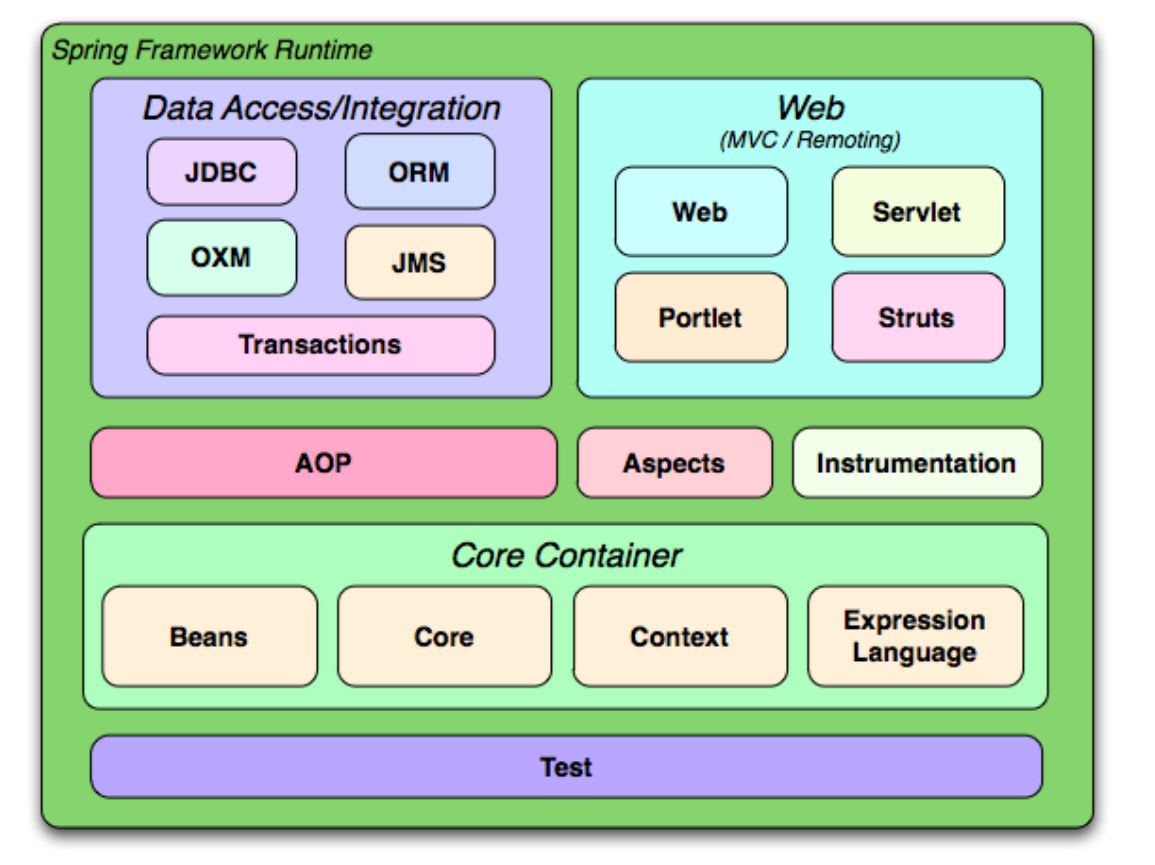
\includegraphics[width=\textwidth]{SpringStructure}
	}
	\caption{Uproszczona Struktura Spring framework. }
	\centering
	\label{fig:springStructure}
\end{figure}


Strukturę Spring najłatwiej przedstawić jako ogromny zbiór konkretnych rozwiązań, każde z nich to osobny moduł, który można wykorzystać. Pozwala to na zmianę projektu aplikacji na każdym etapie jej produkcji np. poprzez określenie innej implementacji za pomocą konfiguracji. Rdzeniem całego szkieletu oraz każdej aplikacji jest Core Container, który zawiera najważniejsze moduły: Beans, Core, Context oraz Expression Language. Moduły Core oraz Beans zapewniają najważniejsze mechanizmy, czyli wstrzykiwanie zależności (ang. Dependency Injection) oraz wiążący się z nim wzorzec architektury odwrócenie sterowania (Inversion of Control). Odpowiadają również za całą logikę związaną z ziarnami (ang. beans) czyli klasami, które zostały odpowiednio adnotowane lub skonfigurowane. Ich instancjonowaniem zajmuje się klasa implementująca interfejs BeanFactory, co pozwala na oddzielenie konfiguracji zależności od jej specyfikacji. Zadaniem modułu Context jest zapewnienie dostępu do obiektów w sposób podobny do specyfikacji JNDI. Opiera się on na wspomnianych już modułach Core oraz Beans, wspiera również standardy Java EE takie jak np. EJB. Ostatnim modułem jest Expression Language, który dostarcza możliwość przeprowadzania zaawansowanych zapytań jak i modyfikacji obiektów w czasie rzeczywistym. 


Aby móc stworzyć aplikację biznesową na tym szkielecie, należy dogłębnie zrozumieć zasadę działania odwrócenia sterowania oraz wstrzykiwania zależności. Oba mechanizmy często są ze sobą utożsamiane, ponieważ są one bazą procesu, w którym każdy obiekt definiuje swoje zależności od innych obiektów poprzez argumenty konstruktora klasy lub za pomocą właściwości klasy ustawianych zaraz po stworzeniu obiektu. Główny kontener wstrzykuje tą zależność podczas tworzenia ziarna. Dzięki temu następuje odwrócenie sterowania, ponieważ to kontener kontroluje tworzenie instancji oraz zależności zamiast ziarna. W procesie tym używane są dwa interfejsy, BeanFactory oraz dziedziczący po nim ApplicationContext. BeanFactory odpowiada za zaawansowaną konfigurację zarządzania obiektem bez względu na jego typ. ApplicationContext rozszerza jego możliwości oraz reprezentuje kontener IoC zarządzający ziarnami. Aby obiekt mógł stać się ziarnem, musi być zarządzany przez kontener. Kontener odczytuje instrukcje dotyczące obiektu z metadanych konfiguracyjnych wyrażonych w formie pliku konfiguracyjnego w formacie XML, adnotacji bądź kodu.



	\begin{figure}[h!]
		\makebox[\textwidth][c]{
			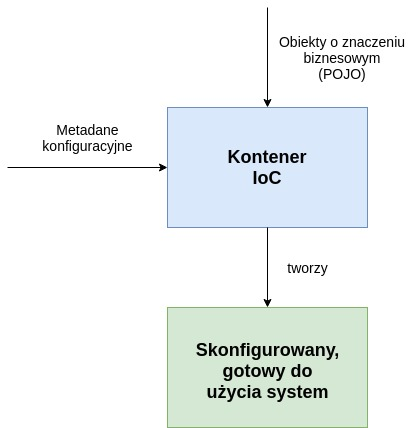
\includegraphics[width=0.55\linewidth]{SpringDiagram1}
		}
		\caption{Kontener Inversion of Control}
		\centering
		\label{fig:inversionOfControl}
	\end{figure}


Odwrócenie sterowania oraz wstrzykiwanie zależności ma kilka bardzo istotnych zalet. Najważniejszą z nich jest zapewnienie luźnego powiązania, ponieważ obiekt nie musi zarządzać zależnościami, znać ich implementację oraz lokalizację. Możemy dzięki temu zmienić implementację zależności bez ingerencji w kod klas, które ją wykorzystują. Testowanie takich obiektów staje się łatwiejsze, ponieważ najczęściej definiujemy zależności poprzez interfejsy lub klasy abstrakcyjne, co pozwala stworzyć atrapę implementacji w testach jednostkowych. Kolejną zaletą tego podejścia jest możliwość łatwego określenia konfiguracji ziarna będącej wzorcem dla stworzenia wielu obiektów. Dzięki adnotacjom możemy wskazać zasięg oraz cykl życia danego ziarna. Domyślnym zachowaniem jest utworzenie tylko jednej instancji zależności zgodnie z wzorcem projektowym Singleton i wstrzyknięcie jej do każdego obiektu zależnego. Istnieje jednak kilka innych możliwości np. określenie ziarna jako prototype w wyniku czego, za każdym wstrzyknięciem kontener tworzy nową instancję. Spring pozwala również na ograniczenie zasięgu ziarna do request, session, application, websocket oraz na stworzenie własnego zasięgu. Poprzez adnotację określamy również cykl życia. Innymi słowy definiujemy jakie akcje mają zostać wykonane w określonych momentach funkcjonowania danego ziarna.





\subsection{Angular 6 framework}
\label{subsec:angularFramework}

W przypadku warstwy prezentacji aplikacji wykorzystany został popularny framework Angular w wersji 6 napisany w języku TypeScript. Jest on przeznaczony do tworzenia aplikacji internetowych typu “Single-Page” czyli aplikacji, w której interakcja z użytkownikiem odbywa się przez dynamiczne nadpisywanie obecnej strony zamiast ładowania nowej. Podejście to sprawia, że aplikacja internetowa zachowuję się bardziej jak aplikacja okienkowa zainstalowana na komputerze tzn. obcowanie użytkownika z aplikacją internetową odbywa się bez zakłóceń w postaci przeładowania strony. Szkielet ten jest obecnie aktywnie wspierany i rozwijany przez firmę Google. 
Architektura szkieletu Angular składa się z kilku kluczowych elementów: modułów (NgModules), komponentów oraz serwisów. Rodzaj elementu jest określany przez odpowiednie metadane w postaci adnotacji umieszczonymi w klasach TypeScript.

Najważniejszym elementem potrzebnym do budowy aplikacji jest moduł, którego zadaniem jest zebranie powiązanego ze sobą kodu i określenie go jako konkretny, funkcjonalny zestaw. Moduł Angulara różni się od modułu JavaScript tym, że deklaruje kontekst kompilacji dla kilku powiązanych ze sobą komponentów oraz łączy te komponenty z innym, powiązanym kodem napisanym w serwisach tak, aby utworzyć konkretną, funkcjonalną jednostkę. Każda aplikacja ma co najmniej jeden moduł nazwany \mbox{AppModule}, który zapewnia mechanizm ładowania przy uruchomieniu aplikacji. Każdy moduł może zaimportować funkcjonalność innego modułu oraz wyeksportować swoją. Zalecaną praktyką jest podzielenie całej aplikacji na kilka modułów, każdy z nich powinien hermetyzować pewną funkcjonalność np. wydzielenie osobnego modułu dotyczącego mechanizmu “routing”. Dzięki temu podejściu projekt skomplikowanej aplikacji jest bardziej czytelny oraz możliwe jest zapewnienie mechanizmu “lazy-loading”, co pozwala na optymalizację wydajności aplikacji poprzez ładowanie konkretnej funkcjonalności dopiero w momencie, gdy jest ona potrzebna. Możemy również w prosty sposób zarządzać zależnościami między modułami oraz podmienić implementacje konkretnego modułu bez dużego wpływu na inne elementy aplikacji.


Następnym elementem aplikacji jest komponent, który definiuje widok połączony z szablonem HTML oraz zawiera dane, logikę biznesową. Każda aplikacja ma co najmniej jeden komponent główny tzw. root, który łączy całą hierarchię komponentów ze strukturą DOM strony. Komponenty mogą również używać serwisów, które zapewniają funkcjonalność nie powiązaną z widokami. Widok komponentu jest zdefiniowany jako szablon podobny do języka HTML oraz jest połączony z klasą TypeScript oznaczoną odpowiednią adnotacją. Wyżej wymieniony szablon oprócz składni HTML zawiera znaczniki charakterystyczne dla Angulara. Pojawia się również kilka przydatnych mechanizmów takich jak powiązanie danych wewnątrz komponentu z danymi w strukturze DOM (ang. data binding), przekształcenie danych przed wyświetleniem za pomocą tzw. “pipes” oraz specjalnych dyrektyw do określenia co ma zostać pokazane i kiedy. Przed wyświetleniem widoku Angular rozpoznaje określone dyrektywy oraz powiązania danych, aby na ich podstawie zmienić strukturę DOM.

Ostatnim głównym elementem jest serwis oraz ściśle z nim związany mechanizm wstrzykiwania zależności. Głównym zadaniem serwisu jest rozwiązanie jednego konkretnego zadania, którego logika oraz dane nie są powiązane z konkretnym widokiem. Dzięki temu do jednego serwisu może się odwoływać wiele komponentów, w wyniku czego nie powtarzamy tego samego kodu. Popularnymi zadaniami są np. pobieranie danych z serwera, ich walidacja oraz rejestracja działań wykonywanych przez aplikację. Aby komponent mógł skorzystać z serwisu musi on zostać odpowiednio wstrzyknięty. Dzieje się to poprzez stworzenie specjalnego iniektora (ang. injector) dla całej aplikacji oraz kilku dodatkowych podczas początkowego ładowania. Iniektor ten tworzy odpowiednie zależności za pomocą specjalnych dostawców (ang. provider), którzy wiedzą jak dana zależność ma zostać stworzona lub dostarczona. Dodatkowo zarządza on kontenerem zależności, dzięki czemu jest w stanie użyć ponownie tej samej instancji w kilku miejscach. Mechanizm wstrzykiwania zależności nie ogranicza się tylko do serwisów, jako zależność może zostać określona np. funkcja, jednak należy pamiętać o zapewnieniu dostawcy. Podczas tworzenia nowej instancji komponentu określone zostają zależności, które dany komponent potrzebuje wzorując się na parametrach konstruktora klasy komponentu. Następnie iniektor sprawdza czy istnieją już instancje potrzebnej zależności. Jeżeli nie istnieje taka instancja odwołuje się do dostawcy w celu stworzenia nowej. Gdy wszystkie zależności są już określone i stworzone, wywołany zostaje konstruktor z nimi jako argumentami.


Warto wspomnieć również o jeszcze jednym bardzo ważnym rozwiązaniu używanym w \mbox{Angular}, czyli routingu. Odpowiada za niego specjalny moduł “Router”, który zapewnia serwis pozwalający zdefiniować nawigację pomiędzy różnymi stanami, hierarchią, widokami w aplikacji. Router mapuje ścieżkę URL tak, aby odwołać się do konkretnego widoku. Użytkownik wykonując różne akcje nie jest przekierowywany do nowej strony, zamiast tego router przechwytuje tą akcję i ładuję konkretny widok. Router jest też w stanie określić, czy dany moduł ma zostać załadowany w zależności od stanu aplikacji. Interpretacja ścieżek URL jest określona w specjalnych regułach nawigacyjnych, które wiążą ścieżkę z konkretnym komponentem. Historia routingu jest również przechowywana, dzięki czemu możliwa jest nawigacja wstecz/wprzód.


\subsection{PostgreSQL}
\label{subsec:postgreSQL}
Do przechowania informacji o użytkownikach oraz projektach została użyta baza danych \mbox{PostgreSQL}. Jest to relacyjno-obiektowy system bazodanowy oparty na licencji "open-source", który rozszerza składnie języka SQL o szereg dodatkowych funkcjonalności usprawniających pracę z danymi o skomplikowanej strukturze. Na przestrzeni wielu lat zyskał reputację systemu niezawodnego oraz rozszerzalnego głównie za sprawą udokumentowanej architektury, integralności danych, zachowania transakcyjności w postaci właściwości ACID oraz szerokiej społeczności, która nieustannie dostarcza innowacyjne i wydajne rozwiązania.


Główną zaletą tego systemu jest jego bardzo obszerna i treściwa dokumentacja oraz mnogość funkcji rozszerzających standard języka SQL. Pierwsza z dodatkowych funkcji to możliwość określenia przechowywanych danych za pomocą licznych typów wbudowanych lub stworzonych przez programistę. Wbudowanych jest około 40, wśród nich warto wymienić kilka naprawdę przydatnych np. json/xml, inet, polygon, money. Następną istotną funkcjonalnością jest zapewnienie integralności danych poprzez możliwość nadania odpowiednich ograniczeń dla danej kolumny np. UNIQUE. Pozwala to na dodatkowe zabezpieczenie przed niepoprawnym zapisem danych. Kolejną bardzo ważna zaletą tego systemu jest skupienie się na wydajności oraz wielowątkowości poprzez liczne systemy wspomagające pracę. Warto wymienić tutaj kilka z nich np. możliwość indeksowania danych w celu szybszego wyszukiwania, optymalizację zapytań do systemu, zapewnienie transakcyjności, współbieżność zapytań typu “read”, partycjonowanie tabel oraz kompilacja wyrażeń w postaci JIT ( ang. Just-in-time). Istotną z punktu widzenia bezpieczeństwa aplikacji jest również funkcjonalność związana z uwierzytelnianiem. PostgreSQL zapewnia wbudowane algorytmy szyfrujące takie jak GSSAPI, SSPI, LDAP, SCRAM-SHA-256, które można wykorzystać w przypadku przechowywania wartościowych danych użytkowników np. hasła dostępu. Oprócz wyżej wspomnianych cech Postgres zapewnia również wyjątkową niezawodność poprzez kilka mechanizmów odzyskiwania informacji po awarii oraz zapobiegania jej.


\chapter{System rekomendacji}

Jednym z problemów występujących przy projektowaniu wygodnej oraz intuicyjnej aplikacji internetowej jest ogromna ilość danych, które trafiają do końcowego użytkownika. W najbardziej popularnych  serwisach internetowych zjawisko to przejawia się w kilku formach np. bardzo duża ilość postów w serwisie Facebook, filmów na YouTube itd. Ogrom informacji docierających do użytkownika sprawia, że jest On przytłoczony oraz ma problem z poruszaniem się po serwisie. Dodatkowo bardzo trudno jest mu w tej sytuacji znaleźć wartościową informację, ponieważ przekazywana mu treść najczęściej nie jest dostosowana do osobistych preferencji, zainteresowań. W celu wyeliminowania tych problemów powstały odpowiednie narzędzia pod ogólną nazwą systemów rekomendacji. Ich głównym zadaniem jest wyszukiwanie i określanie danych o jak największej wartości dla konkretnego zainteresowanego. Spersonalizowana zawartość jest określana na podstawie informacji użytkownika oraz jego akcji wykonanych w przeszłości. Cały proces przygotowania odpowiednich sugestii powinien być w całości zautomatyzowany oraz dawać jak najlepsze efekty w jak najkrótszym czasie. Niestety nie istnieje jedno uniwersalne rozwiązanie, które spełniałoby wyżej wymienione wymagania. Aplikacje różnią się strukturą danych, ilością użytkowników oraz każdy z nich jest nastawiony na uzyskanie innego rezultatu.


Aby sprostać wymagającym oczekiwaniom, powstały odpowiednie metody analityczne pozwalające określić prawdopodobieństwo, z którym dana informacja może być przydatna dla użytkownika. Można je podzielić na trzy główne podejścia:

\begin{itemize}
	\item Content-based filtering
	\item Collaborative filtering
	\item Hybrid filtering
\end{itemize}




\section{Content-based filtering}

Filtrowanie typu Content-based opiera się na rekomendowaniu danych, które są podobne do tych, które użytkownik oznaczył już wcześniej jako interesujące\cite{REC01}. Innymi słowy służy do nauczenia się preferencji użytkownika, a następnie określeniu informacji jak najlepiej spełniających te preferencję. W podejściu tym można określić, które aspekty mają być brane pod uwagę w procesie filtrowania. Aby, skutecznie zaimplementować tą metodę, dane muszą zostać odpowiednio oznaczone w postaci wektora cech \textit{y}. Wektory te są następnie wykorzystywane do określenia preferencji użytkownika.

Istnieje kilka technik stosowanych przy procesie określania modelu do rekomendacji. Jedną z nich jest użycie \textit{Term Frequency} oraz \textit{Inverse Document Frequency} w systemach służących do wyszukiwania informacji. Inne techniki wykorzystują najczęściej metody probabilistyczne w połączeniu z uczeniem maszynowym np. naiwny klasyfikator Bayesa lub drzewa decyzyjne.

\subsection{Term-Frequency, Inverse Document Frequency}
Techniki TF-IDF używane są do określenia, jak ważne jest dane słowo. Stopień ważności jest ściśle powiązane z liczbą występowań słowa w danym tekście, jednak jego wartość maleje wraz z liczbą występowań danego słowa we wszystkich analizowanych dokumentach. Jako przykład niech posłuży słowo \textit{człowiek}. W artykule o zjawiskach biologicznych może zostać użyte dosyć często, dlatego jego wartość wzrasta. Jednak jeżeli dany tekst rozpatrywany jest w kontekście bazy z artykułami o procesach zachodzących w ludzkim ciele, jego wartość powinna mocno zmaleć, ponieważ nie jest ono kluczowe dla użytkownika. Z drugiej strony istnieje inny przypadek, gdy dany tekst występuje w bazie artykułów o różnej tematyce. Ilość występowań tego słowa we wszystkich artykułach jest mała, dlatego jego wartość nie maleje, ponieważ może ono być uznane w tym wypadku za kluczowe.

Term-Frequency może być przedstawione za pomocą poniższego wzoru:
\begin{equation}
 TF_{i,j} = \frac{f_{i,j}}{n_j}
\end{equation}
gdzie:
\begin{itemize}
	\item[] $f_{i,j}$ - częstotliwość występowania słowa $k_i$ w dokumencie $d_j$
	\item[] $n_j$ - liczba wszystkich słów w dokumencie $d_j$
\end{itemize}

W celu określenia popularności słowa we wszystkich dokumentach stosuje się Inverse Document Frequency, wyrażone wzorem:
\begin{equation}
IDF_i = \log{\frac{N}{n_i}}
\end{equation}
gdzie:
\begin{itemize}
	\item[] $N$ - liczba wszystkich dokumentów
	\item[] $n_i$ - liczba dokumentów, w których występuje słowo $k_i$
\end{itemize}

Mając obydwa współczynniki można określić stopień ważności TF-IDF dla słowa $k_i$ w dokumencie $d_j$ określony jako:
\begin{equation}
w_{i,j} = TF_{i,j} \times IDF_i
\end{equation}

Jako przykład rozważmy tekst zawierający 100 słów, w którym słowo \textit{człowiek} pojawia się 3 razy. Współczynnik $TF = \frac{3}{100} = 0,03$. Zakładając, że tekst ten znajduje się w bazie zawierającej 10 milionów artykułów oraz, że słowo \textit{człowiek} występuje w 1000 z nich można obliczyć $IDF = \log{\frac{10000000}{1000}} = 4$. W takim wypadku stopień ważności słowa wynosi $0.12$.

\subsection{Metody probabilistyczne}
Stosowane są w celu określenia prawdopodobieństwa zainteresowania użytkownika $u_i$ danymi $p_j$. Estymacja prawdopodobieństwa opiera się na macierzy \textit{S} w postaci użytkownik-dane. Pośród metod wyliczających prawdopodobieństwo warto wspomnieć o takich jak klasyfikator Bayesa, drzewa decyzyjne oraz sieci neuronowe.  Dodatkowo można też użyć algorytmów uczących w celu rozszerzenia specyfiki rekomendacji np. z określenia co w danej chwili rekomendować do określenia kiedy to rekomendować. Służą do tego algorytmy Association rule, klasteryzacji, drzewa decyzyjne, sieci neuronowe.  

\subsection{Wady i zalety}

Algorytm Content-based filtering posiada kilka wad i zalet ,dzięki którym można określić, czy jest on odpowiedni do danej sytuacji. 

Jedną z jego niewątpliwych zalet jest rozwiązanie problemu tak zwanego ``zimnego startu`` tzn. nie potrzebuje on sporej ilości ocen bezpośrednio od użytkowników aplikacji, aby stworzyć rekomendację. Dzięki temu nadaje się do systemów z małą liczbą użytkowników bądź w przypadku, gdy nie ma potrzeby dzielenia się informacjami między użytkownikami. Inną zaletą jest jego zdolność do uczenia się oraz tworzenia rekomendacji w krótkim czasie. Kolejną z nich jest rozwiązanie problemu stronniczości względem popularności, ponieważ premiuje on dane, które nie są bardzo często używane. 

Jednakże technika ta nie jest idealna i ma swoje wady. Najważniejszą z nich jest zależność od meta danych, co wymusza pewną strukturyzację zawartości. Z tego powodu trudno jest rekomendować niektóre dane np. muzykę. Problem ten znany jest również pod nazwą ograniczonej analizy zawartości, ponieważ ogranicza możliwość wykorzystania nowego typu danych. Innym znanym problemem jest nadmierna specjalizacja zawartości. Oznacza to, że użytkownik może otrzymać rekomendacje bardzo mocno powiązane ze sobą np. w aplikacji rekomendującej filmy mogą zostać wyświetlone wszystkie trzy części Władcy Pierścieni, zamiast jednej oraz dwóch innych pozycji.

\newpage

\section{Collaborative filtering}

Algorytm Collaborative filtering opiera się na założeniu, że jeżeli dwóch użytkowników ma podobne upodobania w obecnym momencie to istnieje duże prawdopodobieństwo, że będą oni również podobne upodobania w przyszłości\cite{REC01}. Jako przykład można podać dwóch użytkowników systemu oceniającego filmy, który dotychczas byli zgodni w ocenach filmów. Jeżeli pierwszy użytkownik dobrze ocenił nowy film, to prawdopodobnie drugi użytkownik również oceni go dobrze. Technika ta jest bardzo przydatna w przypadku, gdy rekomendacja nie powinna być na podstawie dodatkowych informacji o danych bądź użytkownikach. Collaborative filtering dzieli się w zależności od tego czy zastosowano w nim podejście Memory-based bądź Model-based. 

Dla zobrazowania działania tego algorytmu załóżmy kolekcje użytkowników $u_i$ oraz kolekcję filmów $m_j$ gdzie $i = 1,\dots,n$ oraz $j = 1,\dots,m$. Dane muszą zostać zorganizowane w postaci $n \times m$ macierzy $V$, która zawiera oceny filmów przez użytkowników zapisane jako $v_{i,j}$. Gdy użytkownik nie ocenił filmu pole to pozostaje puste.  
$$
V= \left[
\begin{array}{cccc}
	v_{11} & v_{12} & \cdots & v_{1m} \\
	v_{21} &   &   &   \\
	\vdots &   & \ddots  &  \vdots \\
	v_{n1} &   &  \cdots &  v_{nm}  \\
	
\end{array}
\right]
$$

\subsection{Techniki Memory-based}

Można je podzielić na dwie kategorie: User-based lub Item-based. W przypadku User-based szukani są użytkownicy podobni do wybranego użytkownika $u_i$ bazując na podobieństwie w ocenach. Jako rekomendację wysyłane są produkty oznaczone jako interesujące przez wyszukanych użytkowników. Natomiast w podejściu Item-based najpierw szukani są użytkownicy, którzy polubili produkt $m_j$. Jako rekomendowane zostają określone inne produkty polubione przez tych użytkowników.
\newline
\newline


\textbf{User-based Collaborative Filtering}

Jej głównym zadaniem jest identyfikacja osób, które podobnie oceniają te same produkty i zarekomendowanie im nowych pozycji, które zostały dobrze ocenione przez innych użytkowników. Do obliczenia podobieństwa można użyć kilka technik, z czego najpopularniejsze to odległość kosinusowa(\ref{CosineSimilarity}) oraz współczynnik korelacji Pearsona(\ref{PearsonCorrelation}), gdzie $v_ij$ to ocena którą użytkownik $u_i$ dał produktowi $m_j$.

\begin{equation}
\label{CosineSimilarity}
cos(u_i,u_k) = \frac{
\sum_{j=1}^{m} v_{ij}v_{kj}
}{
\sqrt{
\sum_{j=1}^{m}{v^2}_{ij} \sum_{j=1}^{m}{v^2}_{kj} 
}
}
\end{equation}

\begin{equation}
\label{PearsonCorrelation}
S(i,k) = \frac{
	\sum_{j} (v_{ij} - \overline{v_i}) (v_{kj} - \overline{v_k})
}{
	\sqrt{
		\sum_{j} (v_{ij} - \overline{v_i})^2 (v_{kj} - \overline{v_k})^2
	}
}
\end{equation}

Mając już obliczony współczynnik korelacji Pearsona można porównać każdego użytkownika za pomocą poniższej macierzy $n \times n$.

$$
S= \left[
\begin{array}{cccc}
1 & S(1,2) & \cdots & S(1,n) \\
 &  \ddots &   &  S(2,n) \\
 &   & \ddots  &  \vdots \\
 &   &   & 1  \\

\end{array}
\right]
$$

Następnym krokiem jest określenie najbardziej podobnych użytkowników do wybranego użytkownika ($u_i$), które polega na wybraniu $k$-najbliższych sąsiadów, którzy mają najbardziej prawdopodobny współczynnik Pearsona. W następnej kolejności należy zidentyfikować produkty polubione przez tych użytkowników, usunąć z listy produkty, które $u_i$ już widział oraz określić wagę pozostałych produktów. Ostateczna predykcja bazuje na odchyleniu od średniej ocen uzyskanych od najbliższych sąsiadów(\ref{deviation}).

\begin{equation}
\label{deviation}
p(i,k) = \overline{v_i} + 
\frac{
	\sum_{i=1}^{n} (v_{ij} - \overline{v_k}) \times S(i,k)
}{
	\sum_{i=1}^{n} S(i,k)
}
\end{equation}
 

\textbf{Item-based Collaborative Filtering}

Algorytm ten w swoim działaniu jest zupełnie różny od opisanego wcześniej User-based Collaborative Filtering, ponieważ jego zadaniem jest określenie podobieństwa dwóch produktów $m_j$ oraz $m_i$. Podobieństwo jest wyliczane na podstawie odległości kosinusowej bądź współczynnika korelacji Pearsona.

W przypadku odległości kosunusowej(\ref{CosineSimilarity}), dwa produkty są określano jako wektory w n wymiarowej przestrzeni użytkowników, gdzie różnica między ocenami użytkowników nie jest brana pod uwagę. 

Natomiast biorąc współczynnik korelacji Pearsona(\ref{PearsonCorrelationSecond}), ważnym krokiem jest wyizolowanie przypadku, gdzie użytkownicy ocenili jednocześnie produkty $m_j$ oraz $m_l$. W poniższym równaniu $U$ oznacza użytkowników, którzy ocenili obydwa produkty. 

\begin{equation}
\label{PearsonCorrelationSecond}
S(i,k) = \frac{
	\sum_{i \in U} (v_{ij} - \overline{v_j}) (v_{il} - \overline{v_l})
}{
	\sqrt{
		\sum_{i \in U} (v_{ij} - \overline{v_j})^2 
	}
	\sqrt{
	\sum_{i \in U} (v_{il} - \overline{v_l})^2
	}
}
\end{equation}

Analogicznie do techniki User-based otrzymujemy macierz o wymiarach $m \times m$, która pokazuje podobieństwo między wszystkimi produktami. Na podstawie pozycji, które dany użytkownik wcześniej ocenił wybierane są nowe, które mają największy współczynnik podobieństwa oraz nie zostały wcześniej wybrane przez użytkownika.

\newpage

\subsection{Techniki Model-based}

Służą do budowania modelu przeznaczonego dla algorytmów uczenia maszynowego oraz eksploracji danych. W swoim działaniu bazują na bardzo popularnej metodzie uczenia nienadzorowanego tzn. faktoryzacji macierzy. Pozwala na redukcję wymiaru macierzy oraz nauczenie się preferencji użytkownika na podstawie ocen tak, aby określić predykcję na temat oceny innych przedmiotów przez niego. Obecnie trzy najpopularniejsze techniki to Principal Component Analysis, Probabilistic Matrix Factorization, Singular Value Decomposition. 

\bigskip

\textbf{Principal Component Analysis}

Używa transformacji ortogonalnej w celu redukcji wymiarów danych. Głównym jej celem jest transformacja zestawu zmiennych, które mogą być ze sobą powiązane w zestaw nowych, niepowiązanych wektorów tzw. głównych komponentów. Wiąże się to z pewną stratą informacji, ponieważ zestaw głównych komponentów jest mniejszy niż wejściowy zestaw zmiennych. Jednakże konstrukcja tej metodologii pozwala zachować maksymalną wariancję oraz sprawia, że metoda najmniejszych kwadratów jest bardziej precyzyjna. Każdy komponent zawiera procentową wartość wariancji. Dzięki temu można zredukować wymiary poprzez wybranie jaką wariancję należy rozpatrywać.

\bigskip


\textbf{Probabilistic Matrix Factorization}


Jest metodą probabilistyczną, używającą obserwacji szumu Gaussa. Macierz przedmiotów użytkownika składa się z dwóch macierzy niskiego rzędu, jedna dla użytkowników, a druga dla przedmiotów. Biorąc ponownie przykład z filmami załóżmy, że $n$ oznacza liczbę użytkowników, $m$ liczbę filmów, $v_{i,j}$ oznacza ocenę dla filmu $p_j$ wystawioną przez użytkownika $u_i$, a $U_i$ oraz $P_j$ reprezentują zbiór wektorów cech odpowiednio dla użytkowników oraz filmów. Następnie definiując przestrzeń obserwowanych ocen jako $V \in R^{n \times m}$, a dystrybucję użytkowników oraz filmów jako $U \in R^{d \times n}$ oraz $P \in R^{d \times m}$ możemy określić warunkową dystrybucję wzorem:

\begin{equation}
p(V|U,V, \sigma^2) = \prod_{i=1}^{n} \prod_{j=1}^{m} [\eta(V_{ij} | U^{T}_i P_j \sigma^2) ]^{I_{ij}}
\end{equation}
\begin{equation}
p(U|\sigma^2) = \prod_{i=1}^{n} \eta (U_i | 0, \sigma^{2}_U I)
\end{equation}
\begin{equation}
p(P|\sigma^2) = \prod_{j=1}^{m} \eta (V_j | 0, \sigma^{2}_P I)
\end{equation}

gdzie:
\begin{itemize}
	\item[] $\eta(x|\mu, \sigma^2)$ - oznacza dystrybucję Gaussa ze średnią $\mu$ oraz wariancją $\sigma^2$
	\item[] $I_{ij}$ - jest wskaźnikiem wynoszącym 1, gdy użytkownik $u_i$ ocenił film $p_j$ lub 0 w przeciwnym wypadku
\end{itemize}
\newpage

\textbf{Singular Value Decomposition}


Podejście to jest najczęściej wykorzystywane i może zostać wyrażone ogólnym równaniem $ X = U \times S \times V^t$. $X$ to macierz użytkownik-przedmiot o wymiarach $n \times m$, $U$ to macierz o wymiarach $n \times r$ reprezentująca wektory cech dotyczące użytkowników, $V^t$ oznacza macierz ortogonalną o wymiarach $r \times m$ reprezentującą wektory cech dotyczące przedmiotów, a macierz diagonalna $S$ o wymiarach $r \times r$ zawiera nie ujemne wartości na przekątnej i jest znana jako. Predykcja wykonana poprzez iloczyn wszystkich wymienionych macierzy(\ref{svd}).

\begin{equation}
\label{svd}
	 X_{n \times m} = U_{n \times r} \times S_{r \times r} \times V^{t}_{r \times m}
\end{equation}

\subsection{Wady i zalety}

Rozpatrując wady i zalety podejścia Collaborative Filtering należy najpierw osobno rozpatrzeć techniki Memory-based oraz Model-based. 

Algorytmy User-based oraz Item-based Collaborative Filtering są bardzo użyteczne w większości wypadków, ponieważ są stosunkowo proste w implementacji, a rezultaty mogą być w większości zadowalające. Jednakże istnieją dwa poważne ograniczenia, które dotyczą każdej z nich. Pierwsze ograniczenie dotyczy minimalnej ilości ocen przedmiotu. Jeden z możliwych scenariuszy zakłada, że oceniany przedmiot jest nowy lub mało popularny, w wyniku czego posiada nie wiele ocen. Powoduje to sporą trudność w określeniu rekomendacji przez algorytm najbliższego sąsiada, jego dokładność mocno maleje. Innym problemem jest skalowalność algorytmu w obliczu coraz to większej ilości danych, ponieważ zapotrzebowanie na moc obliczeniową mocno wzrasta.

Z drugiej strony istnieją techniki Model-based, które radzą sobie znacznie lepiej z wyżej wymienionymi ograniczeniami. Starają się one znaleźć relację pomiędzy przedmiotami-użytkownikami, a następnie stworzyć rekomendację poprzez porównanie tych relacji. Ich wadami z kolei są słaba wydajność, złożoność obliczeniowa oraz wysoka podatność na zjawisko nadmiernego dopasowania przez stosowanie algorytmu faktoryzacji macierzy. 

Istnieją również inne ograniczenia Collaborative Filtering takie jak problem zimnego startu. Polega on na braku odpowiedniej ilości informacji o nowym użytkowniku, co nie pozwala stworzyć dla niego rekomendacji. Problem ten może się również pojawić w przypadku braku odpowiedniej ilości danych, za pomocą następuje porównanie. W takim wypadku lepszym wyjściem byłoby zastosowanie jednego z podejść hybrydowych. 

\section{Hybrid filtering}


Metody hybrydowe polegają na połączeniu metod Content-based filtering oraz Collaborative filtering tak, aby wyeliminować większość wad pojawiających się podczas używania tylko jednej z nich \cite{REC01}. Istnieje kilka kombinacji metod hybrydowych, które mogą być podzielone na 4 grupy:
\begin{itemize}
	\item osobna implementacja Content-based oraz Collaborative, a następnie połączenie ich predykcji 
	\item dodanie charakterystyki Content-based do modelu Collaborative poprzez użycie wszystkich technik w obrębie Collaborative Filtering z tą różnicą, że każdy użytkownik jest brany pod uwagę
	\item dodanie charakterystyki Collaborative do modelu Content-based poprzez użycie np. techniki faktoryzacji macierzy w profilu użytkownika utworzonego przez Content-based
	\item opracowanie jednego systemu rekomendacji, który używa charakterystyki zarówno Content-based oraz Collaborative w różnym stopniu
\end{itemize}

\chapter{Projekt aplikacji}

W ramach części praktycznie pracy wykonano aplikację internetową \mbox{\textit{ProjectSHARE}}. Podczas implementacji skupiono się głównie nad stworzeniem prostego, wygodnego interfejsu użytkownika oraz nad dostosowaniem wyświetlanej treści do użytkownika. Aby osiągnąć zamierzone rezultaty, w procesie wytwarzania aplikacji wykorzystano metodologię zwinną oraz związane z nią krótkie iteracje, ustalenie wymagań na podstawie tzw. \textit{User Stories} oraz estymację kosztów wytworzenia funkcjonalności za pomocą techniki \textit{Planning Poker}.

\section{Założenia}

Główne założenia towarzyszące projektowaniu aplikacji to: prostota interfejsu
użytkownika, łatwe wyszukiwanie projektów, rekomendacja projektów wykorzystująca informacje o użytkowniku oraz odgórne
ograniczenie ilości udostępnianych informacji o projekcie. Część aplikacji wzorowana jest na kilku
rozwiązaniach wykorzystywanych w bardzo popularnych serwisach, np. ograniczona liczba
znaków stosowana w aplikacji Twitter oraz prosta mechanika oznaczania jako obserwowane. W systemie
rekomendacji wykorzystywany jest algorytm uczenia Content-based filtering, który na podstawie tagów projektów oznaczonych jako obserwowane, wyszuka w bazie danych odpowiednie przedsięwzięcia.

Wyżej wymienione założenia pozwalają na stworzenie platformy nadającej się dla
każdego, ponieważ wyświetlane projekty są dostosowane do użytkownika. Dodatkowo autor ukrywa całą implementacje i szczegóły
swojej pracy, ponieważ istnieje odgórne ograniczenie znaków w opisie projektu. Dzięki temu
założeniu możliwa jest również współpraca bezpośrednio z przedsiębiorstwami, które mogą udostępnić
jedynie ogólny opis swojego produktu. Daje to dodatkowe możliwości takie jak np.
darmowa reklama lub rekrutacja innych użytkowników. Jednocześnie
branża w której autor się obraca nie ma tak wielkiego znaczenia jak w przypadku innych
repozytorium, ponieważ projekty oznaczane są odpowiednimi tagami, a serwis wyszukuje
je wedle upodobań autora.

\bigskip
\bigskip
\bigskip
\bigskip

\section{Specyfikacja wymagań}

Wymagania zostały podzielone na dwie kategorie: biznesowe oraz technicznie. Biznesowe oznaczają wymaganie sprecyzowane przez klienta w postaci historyjek użytkownika. Są one krótkim opisem cech i właściwości systemu z perspektywy potrzeb użytkownika. Mają one ujednoliconą strukturę w postaci ,,Jako ... chcę ..., ponieważ ...''.  Ustala się je we współpracy z klientem tak, aby uwzględnić w nich najważniejsze aspekty np. łatwość oszacowania kosztu wytworzenia, wartość biznesowa, określenie kryteriów akceptacji, możliwość wykonania w obrębie jednej iteracji. Ich największą zaletą jest uspójnienie wizji, określenie pożądanego efektu oraz minimalizacja ryzyka wystąpienia nieporozumienia. Techniczne wymagania są natomiast ustalane przez zespół programistów na podstawie wymagań biznesowych. Z reguły nie są one prezentowane klientowi, ponieważ są one zrozumiałe dla konkretnej grupy osób. Ich zadaniem jest określenie konkretnych elementów systemu, które należy wykonać. W przypadku metodyki agile powinny one być uzupełnieniem wymagań biznesowych oraz podlegać ciągłej zmianie \cite{AGI01}. Ich niewątpliwą zaletą jest możliwość pokazania większej abstrakcji systemu, niż w przypadku historyjki użytkownika. Jedno wymaganie techniczne może odnosić się do kilku scenariuszy wynikających z historyjek biznesowych, dzięki czemu koszt jest mocno redukowany. Inną zaletą ich stosowania jest większa przejrzystość dla programisty. 

\bigskip

Dla aplikacji \mbox{\textit{ProjectSHARE}} wyróżniono następujące wymagania biznesowe w postaci \textit{User Stories}:
\begin{itemize}
	\item[$\bullet$] Jako użytkownik chciałbym mieć możliwość logowania za pomocą adresu e-mail, ponieważ jest to wygodny standard w wielu aplikacjach internetowych
	\item[$\bullet$] Jako użytkownik chciałbym mieć możliwość tworzenia inicjatyw publicznych oraz łączenia się w zespoły, ponieważ znalezienie osób chętnych do realizacji projektu jest dzięki temu prostsze i szybsze
	\item[$\bullet$] Jako użytkownik chciałbym mieć możliwość tworzenia inicjatyw prywatnych, tak abym mógł sam zdecydować, kto dołączy do projektu 
	\item[$\bullet$] Jako użytkownik chciałbym móc wysyłać zaproszenia do konkretnych użytkowników, tak aby mogli dołączyć do projektu prywatnego
	\item[$\bullet$] Jako użytkownik chciałbym, aby wyświetlały mi się projekty dostosowane do moich zainteresowań, ponieważ zaoszczędzę w ten sposób czas spędzony na szukaniu interesujących projektów
	\item[$\bullet$] Jako użytkownik chciałbym mieć możliwość wygodnego przeglądania innych projektów
	\item[$\bullet$] Jako użytkownik chciałbym oznaczyć projekt jako obserwowany, ponieważ będę miał możliwość szybkiego powrotu do niego
	\item[$\bullet$] Jako użytkownik chciałbym mieć możliwość komunikacji z innym użytkownikiem, ponieważ wymiana informacji jest jednym z kluczowych aspektów przy pracy w projekcie oraz przy rekrutacji innych użytkowników do projektu
	\item[$\bullet$] Jako użytkownik chciałbym, aby powiadomienia przychodziły mi na maila, ponieważ mógłbym zostać powiadomiony o jakiejś akcji bez wchodzenia do aplikacji
	\item[$\bullet$] Jako użytkownik chciałbym móc przeglądać profil innego użytkownika, ponieważ daje mi to możliwość weryfikacji jego aktualnych działań oraz projektów
	\item[$\bullet$] Jako użytkownik chciałbym móc wyszukać projekt po tagach, ponieważ jest to bardziej precyzyjne.
\end{itemize}

\bigskip

Na podstawie wymagań biznesowych wyróżniono następujące wymagania techniczne w postaci elementów systemu:
\begin{itemize}
	\item[$\bullet$] Panel logowania za pomocą email
	\item[$\bullet$] Formularz rejestracji
	\item[$\bullet$] Panel służący do wyświetlania profilu użytkownika
	\item[$\bullet$] Panel wyświetlający rekomendowane projekty
	\item[$\bullet$] Panel wyświetlający listę projektów obserwowanych
	\item[$\bullet$] Komunikator
	\item[$\bullet$] Panel z informacjami o projekcie
	\item[$\bullet$] Formularz tworzenia projektu
	\item[$\bullet$] Wyszukiwarka projektów
	\item[$\bullet$] Algorytm Content-based filtering dla systemu rekomendacji
	\item[$\bullet$] Powiadomienia email
\end{itemize}

\section{Realizacja aplikacji}

Proces implementacji został podzielony na 4 dwutygodniowe iteracje. Ilość iteracji była ograniczona przez ustalony z góry termin osiągnięcia tzw. produktu o minimalnej wartości. Aplikacja spełnia założenia tego typu produktu w przypadku, gdy oferuje najważniejsze funkcjonalności określone przez klienta. Aby to osiągnąć przeprowadzono najpierw estymację kosztu wyprodukowania wszystkich historyjek użytkownika za pomocą techniki \textit{Planning Poker}. Wartości przydzielane poszczególnym historyjką zostały ustalone za pomocą kolejnych liczb ciągu Fibonacciego. Jako zdolność zespołu na każdą iterację przyjęto wartość 30, co również służyło jako punkt odniesienia podczas estymacji kosztów. Poniżej znajduje się tabela zawierająca skrócony opis wszystkich historyjek oraz przydzielone do nich \textit{story points}.


\begin{figure}[h!]
	\makebox[\textwidth][c]{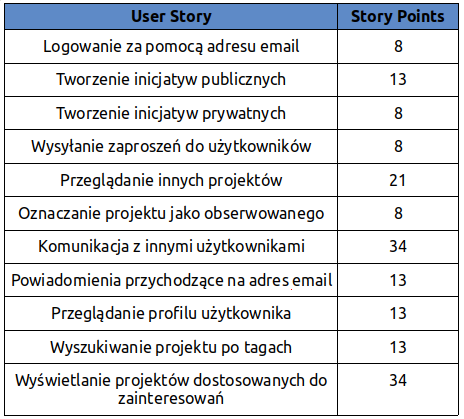
\includegraphics[scale=0.6]{UserStories}
	}
	\caption{Tabela historyjek użytkownika wraz z przydzielonymi punktami}
	\centering
\end{figure}

Suma wszystkich punktów wynosi 173. Biorąc pod uwagę zdolność zespołu oraz liczbę iteracji możliwe jest spełnienie tylko 120 punktów, dlatego w następnym kroku określono historyjki najważniejsze z punktu widzenia klienta. Mając te dane przystąpiono do planowania poszczególnych iteracji oraz historyjek które mają zostać zaimplementowane w każdej z nich. Tak powstały plan był głównym artefaktem podczas procesu implementacji, który jasno wyznaczał jakie zadanie mają zostać spełnione w danej iteracji. Zgodne z metodologią zwinną ulegał on pewnym zmianą wraz z postępami oraz zmieniającymi się wymaganiami co jest, jednak przez dobre oszacowanie kosztów zmiany były nieznaczne. 
\bigskip

\begin{figure}[h!]
	\makebox[\textwidth][c]{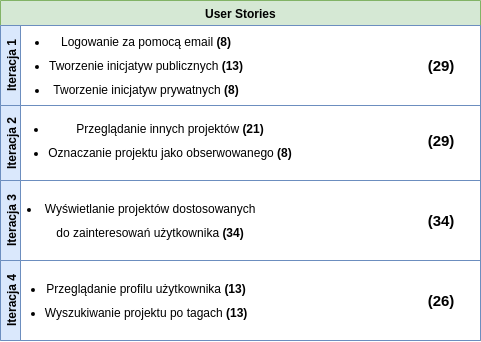
\includegraphics[scale=0.6]{Iteracje}
	}
	\caption{Iteracje wraz z przydzielonymi historyjkami}
	\centering
\end{figure}

\section{Model bazy danych}
Struktura bazy danych została zaprojektowana tak, aby implementacja założonych  funkcjonalności była jak najprostsza. Jest ona jednocześnie zwarta i przejrzysta, co pozwala na dalszą jej rozbudowę oraz dodanie nowych tabel w przypadku potrzeby implementacji nowej funkcjonalności. Poniżej znajduje się diagram ERD przedstawiający zależności między tabelami.
\begin{figure}[h!]
	\makebox[\textwidth][c]{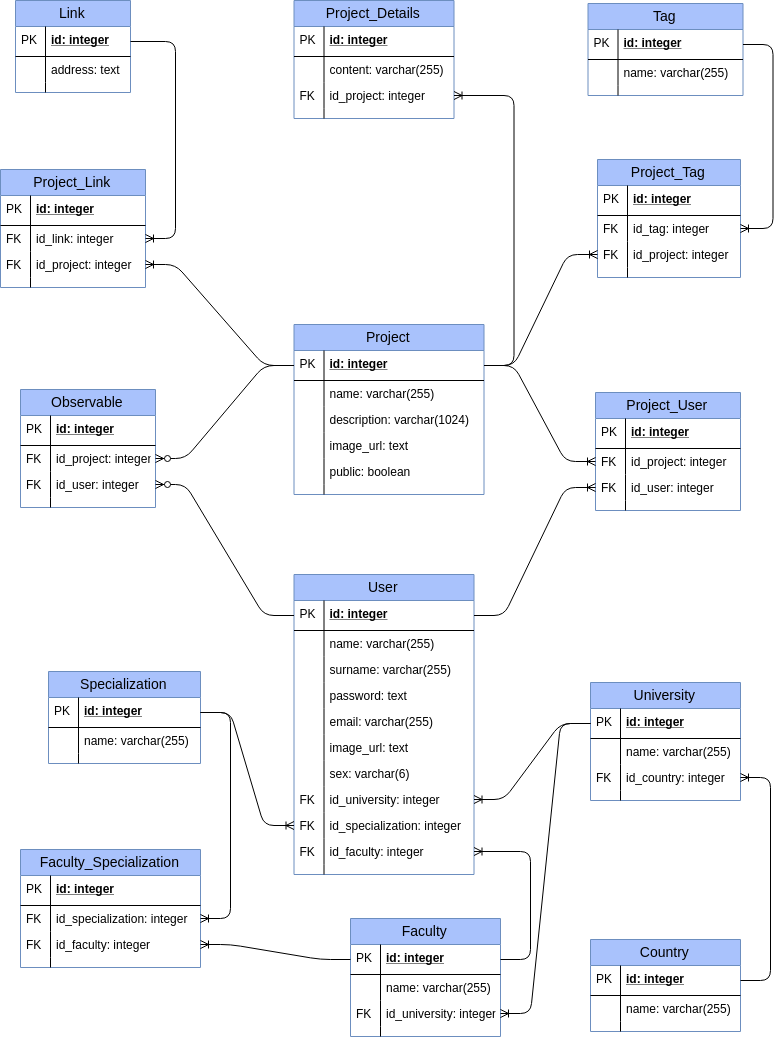
\includegraphics[scale=0.5]{Database}
	}
	\caption{Diagram ERD bazy danych}
	\centering
\end{figure}


\section{Architektura systemu}

Aplikacja składa się z 3 głównych elementów: bazy danych, warstwy back-end w postaci Representational State Transfer Application Programming Interface oraz aplikacji internetowej typu Single Page. Każdy z wyżej wymienionych elementów stanowi osobną całość w systemie, co pozwala na niezależne rozwijanie każdej z nich. Najniższą warstwa to warstwa bazy danych, która jest odpowiedzialna za przechowywanie informacji. Do zarządzania bazą danych oraz zasobami służy REST API, które udostępnia wybrane operację poprzez protokół HTTP. Każdy zasób posiada unikalną ścieżkę, dzięki której można się do niego odwołać oraz wykonać operacje Create, Read, Update, Delete. Udostępniane dane są w formacie JavaScript Object Notation. W przypadku tworzenia danego zasobu, dane potrzebne do stworzenia obiektu również są w formacie JSON. Elementem systemu służącym jako interfejs użytkownika jest aplikacja internetowa typu Single Page, która pozwala na interakcję użytkownika z systemem bez opóźnień wynikających z przeładowania strony. Opiera się na asynchronicznej komunikacji z wspomnianym wyżej REST API. Dodatkowo separuje logikę związaną z wyświetlaniem informacji użytkownikowi.
\bigskip

\begin{figure}[h!]
	\makebox[\textwidth][c]{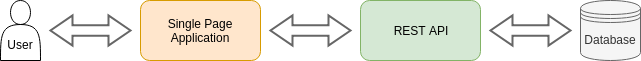
\includegraphics[scale=0.6]{SimpleArchitecture}
	}
	\caption{Uproszczona architektura systemu}
	\centering
\end{figure}

\bigskip

\subsection{Struktura REST API}

REST API do wykonania operacji na odpowiednim zasobie wykorzystuje strukturę drzewiastą, która jest reprezentowana przez ścieżki URL. Zgodnie z przyjętą konwencją, każdy punkt końcowy reprezentuje zasób jako rzeczownik w liczbie mnogiej. Aby dostać się do niego należy wysłać odpowiednie żądanie. Jeżeli jest ono prawidłowe, w odpowiedzi przesyłany jest najczęściej obiekt w formacie JSON reprezentujący zasób oraz kod statusu HTTP. Do poszczególnych zasobów powinno się odwoływać od najbardziej ogólnego elementu do najbardziej szczegółowego. Dla każdej ścieżki mogą zostać zaimplementowane cztery metody HTTP: GET, POST, PUT, DELETE. Reprezentują one operację typu CRUD, które można wykonać na danym zasobie. Dodatkowo można zdefiniować, które parametry HTTP Headers są wymagane w żądaniu, co pozwala na zabezpieczenie dostępu do zasobu poprzez np. autoryzację za pomocą tokenów. Poniżej znajdują się diagramy reprezentujące zaimplementowane punkty końcowe ścieżki dla aplikacji \mbox{\textit{ProjectSHARE}} wraz z możliwymi operacjami.

\bigskip
\bigskip
\bigskip
\bigskip
\bigskip
\bigskip
\bigskip
\bigskip
\bigskip
\bigskip
\bigskip\bigskip
\bigskip\bigskip
\bigskip\bigskip
\bigskip\bigskip
\bigskip


\begin{figure}[h!]
	\makebox[\textwidth][c]{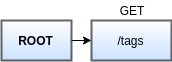
\includegraphics[scale=0.6]{TagsEndpoints}
	}
	\caption{Ścieżki URL do wykonania operacji na tagach}
	\centering
\end{figure}



\begin{figure}[h!]
	\makebox[\textwidth][c]{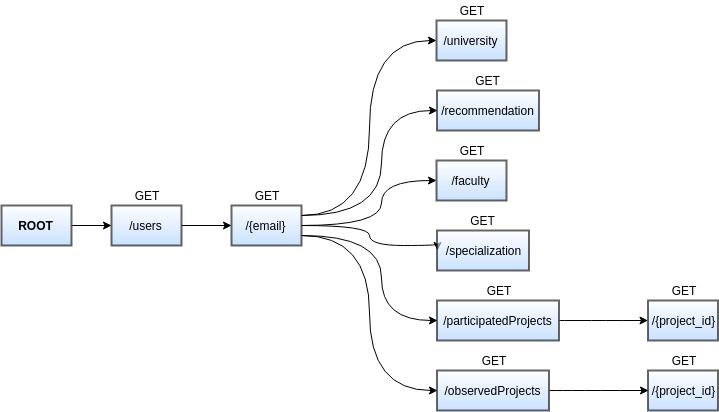
\includegraphics[scale=0.55]{UserEndpoints}
	}
	\caption{Ścieżki URL do wykonania operacji na użytkownikach}
	\centering
\end{figure}


\begin{figure}[h!]
	\makebox[\textwidth][c]{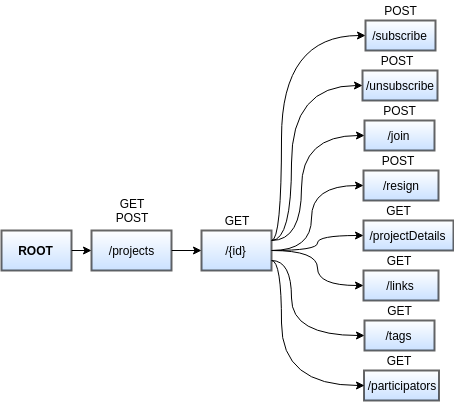
\includegraphics[scale=0.6]{ProjectsEndpoints}
	}
	\caption{Ścieżki URL do wykonania operacji na projektach}
	\centering
\end{figure}


\begin{figure}[h!]
	\makebox[\textwidth][c]{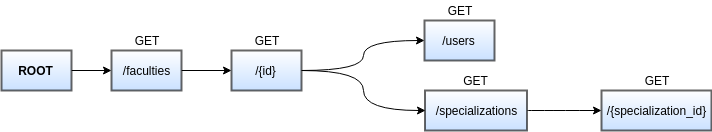
\includegraphics[scale=0.5]{FacultiesEndpoints}
	}
	\caption{Ścieżki URL do wykonania operacji na wydziałach}
	\centering
\end{figure}

\begin{figure}[h!]
	\makebox[\textwidth][c]{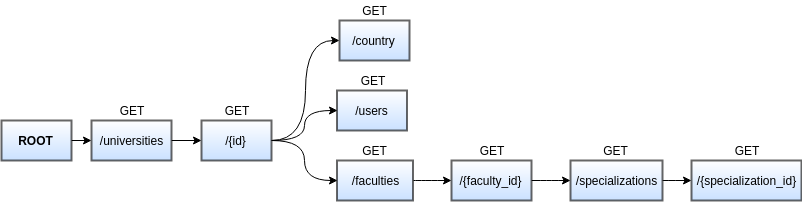
\includegraphics[scale=0.5]{UniversitiesEndpoints}
	}
	\caption{Ścieżki URL do wykonania operacji na uniwersytetach}
	\centering
\end{figure}

\begin{figure}[h!]
	\makebox[\textwidth][c]{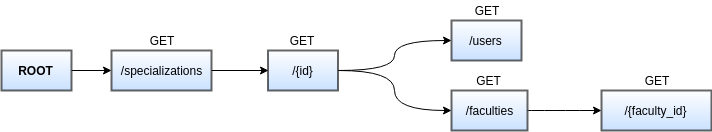
\includegraphics[scale=0.5]{SpecializationsEndpoints}
	}
	\caption{Ścieżki URL do wykonania operacji na specjalizacjach}
	\centering
\end{figure}





\subsection{Architektura aplikacji internetowej}

Aplikacja internetowa \mbox{\textit{ProjectSHARE}} składa się z kilku komponentów wydzielających logikę związaną z konkretną funkcjonalnością. Każdy komponent jest dynamicznie wstrzykiwany w zależności od przypisanej do niego ścieżki URL, co zwiększa wydajność aplikacji oraz poprawia komfort użytkowania. Za poruszanie się po ścieżkach oraz dobór odpowiednich komponentów odpowiedzialny jest specjalny \textit{router}, będący wbudowanym narzędziem szkieletu Angular. Informację o tym, który komponent jest przypisany do jakiej ścieżki oraz czy może zostać w danym momencie wyświetlony są przechowywane w wydzielonym module \textit{app-route}. Za komunikację z REST API odpowiedzialne są następujące serwisy: \textit{UserService, ProjectService, TagService, UserAuthService}. Każdy serwis oznaczone adnotacją \textit{@Injectable()} może zostać wstrzyknięty do komponentu poprzez konstruktor. Ich głównym zadaniem jest implementacja odpowiednich metod wywołujący określone operacje na zasobach REST API. Serwisy te również przekazują asynchronicznie dane do konkretnych komponentów korzystając z modelu komunikacji Publisher-Subscriber. Dodatkowo istnieje jeszcze jeden serwis \textit{AuthGuardService} implementujący interfejs \textit{CanActivate}. Pozwala on na zdefiniowanie metody zwracającej informację o tym, czy dany komponent może zostać wyświetlony w zależności od tego, czy użytkownik jest zalogowany czy też nie. Jest on stosowany tylko we wspomnianym wyżej wymienionym module \textit{app-route}.

\begin{figure}[h!]
	\makebox[\textwidth][c]{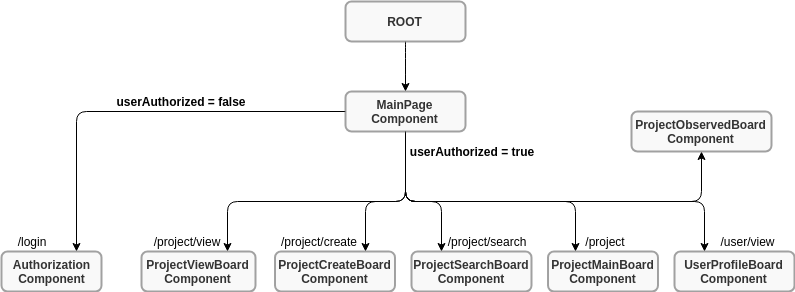
\includegraphics[scale=0.5]{SPAStructure}
	}
	\caption{Struktura komponentów wraz z odpowiadającymi im ścieżkami}
	\centering
\end{figure}


\section{Interfejs użytkownika}

Podczas projektowania interfejsu użytkownika kierowano się głównie wygodą interakcji użytkownika z aplikacją oraz starano się stworzyć go jasnym i przejrzystym. Wzorowano się na najpopularniejszych serwisach dostępnych w internecie oraz stylu projektowania aplikacji internetowych o nazwie \textit{Material Design}. Do wygodnego poruszania się pomiędzy przygotowanymi widokami służy pasek nawigacyjny zawierający nazwy dostępnych widoków. Pasek ten jest zawsze w jednym miejscu tak, aby użytkownik miał do niego stały dostęp. W celu zapewnienia wygody użytkowania na każdym urządzeniu zastosowano odpowiednie pozycjonowanie. Dla urządzeń mobilnych zmieniono również zachowanie niektórych elementów np. rozwijany pasek nawigacyjny zamiast stałego miejsca u góry strony. 

Po wejściu na główną stronę aplikacji można zalogować się do systemu poprzez specjalny formularz logowania podając adres email oraz hasło. 



\begin{figure}[h!]
	\makebox[\textwidth][c]{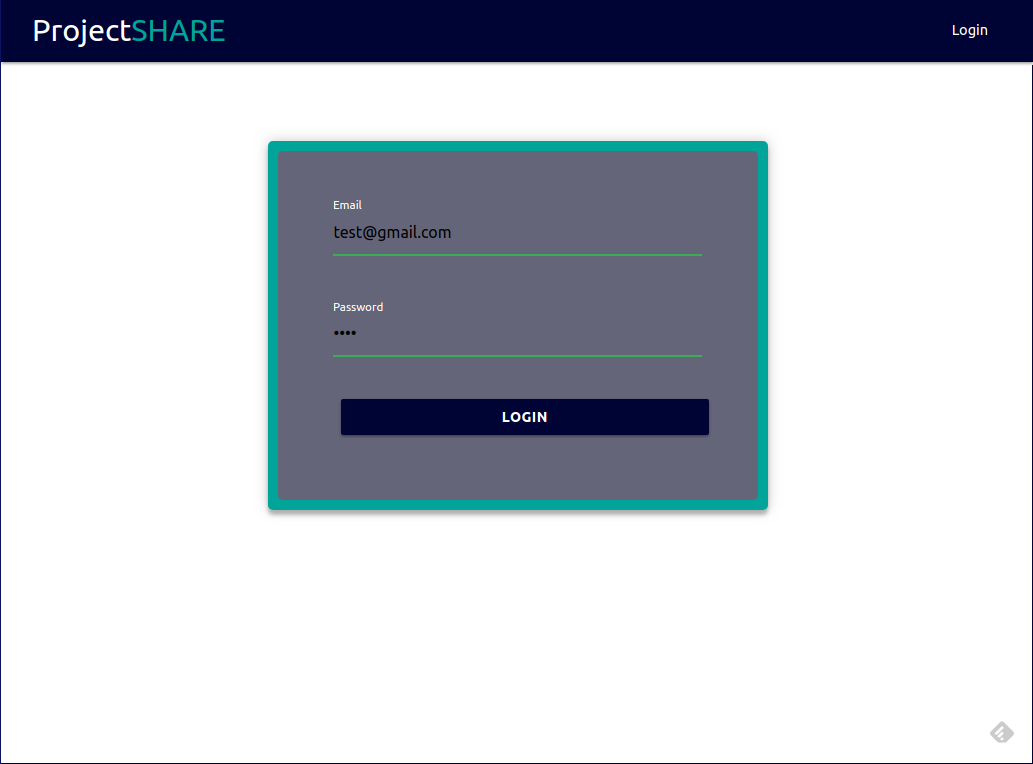
\includegraphics[scale=0.3]{screenLogin}
	}
	\caption{Formularz logowania}
	\centering
\end{figure}


Po zalogowaniu następuje przekierowanie na główny panel z projektami. Jest to widok zawierający 5 najbardziej polecanych projektów dla danego użytkownika, wybranych przez system rekomendacji. Użytkownik aplikacji może przeczytać skrócony opis danego projektu, powiększyć zdjęcie go reprezentujące oraz przejść do rozszerzonego opisu projektu. Od momentu zalogowania, po lewej stronie umieszczona została lista z projektami obserwowanymi, na której widać nazwy wraz ze zdjęciami. Po kliknięciu na dany projekt wysuwa się krótkie zdanie opisujące oraz przekierowanie do rozszerzonego opisu. Jest on zawsze dostępny tak, aby spełnić wymagania klienta i szybkim dostępie do projektów obserwowanych.

\begin{figure}[h!]
	\makebox[\textwidth][c]{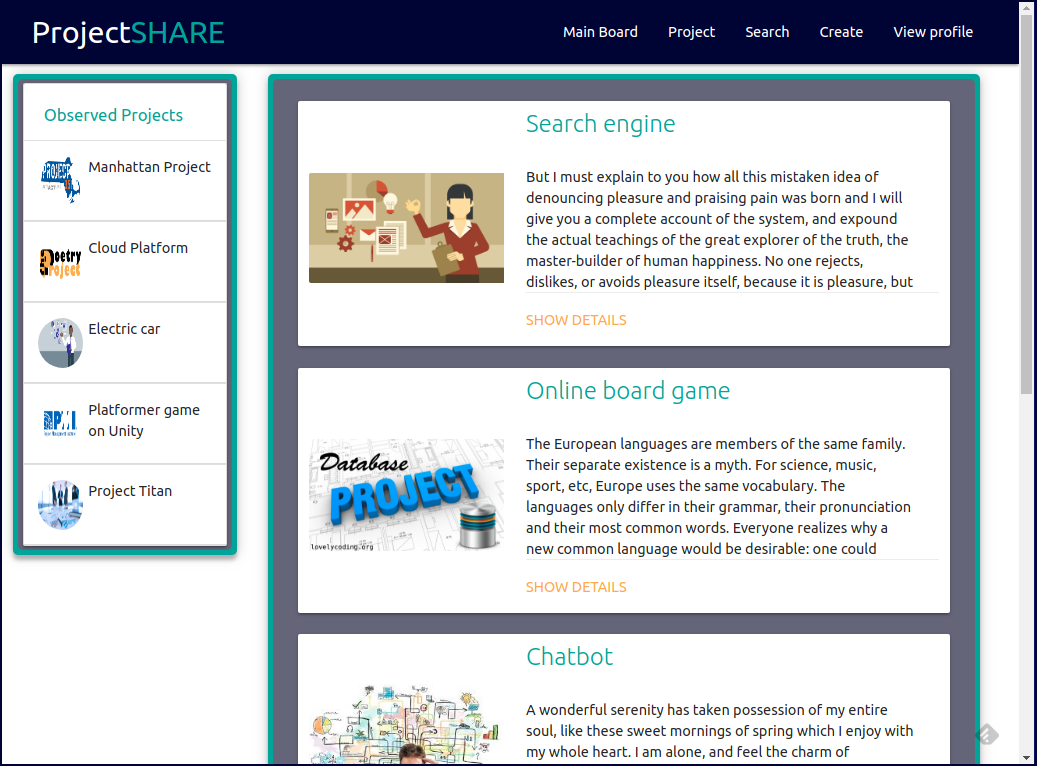
\includegraphics[scale=0.35]{screenMainBoard}
	}
	\caption{Widok z polecanymi projektami}
	\centering
\end{figure}

Kolejnym panelem jest widok rozszerzonego opisu projektu. W pierwszej kolejności przedstawiony jest tytuł, zdjęcie oraz dwa przyciski \textit{subscribe/unsubscribe}, \textit{join/resign}. Za pomocą pierwszego przycisku możemy dodać lub usunąć projekt do listy obserwowanych, a za pomocą drugiego możemy dołączyć do projektu albo z niego zrezygnować. Poniżej znajduje się tekstowy opis ograniczony do 1024 znaków oraz lista zawierająca szczegóły. Następnie wyświetlana jest karta linków związanych z projektem, lista uczestników oraz tagi, którymi dany projekt jest oznaczony.

\begin{figure}[h!]
	\makebox[\textwidth][c]{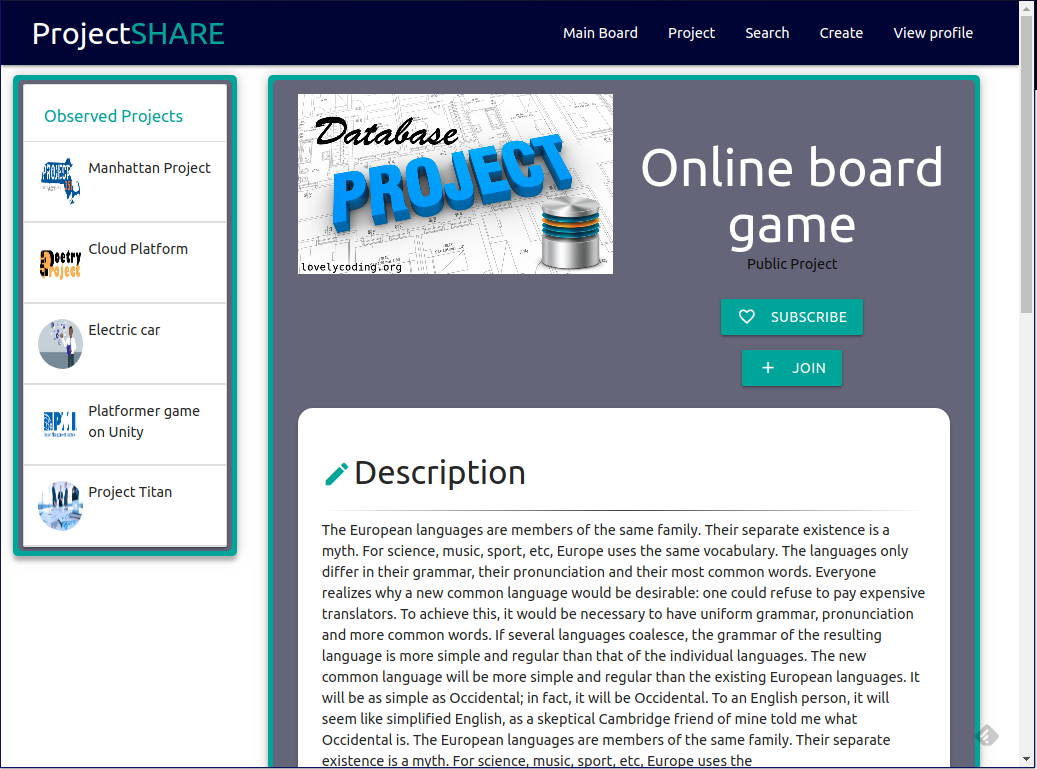
\includegraphics[scale=0.35]{screenProject1}
	}
	\caption{Widok rozszerzonego opisu projektu cz.1}
	\centering
\end{figure}

\begin{figure}[h!]
	\makebox[\textwidth][c]{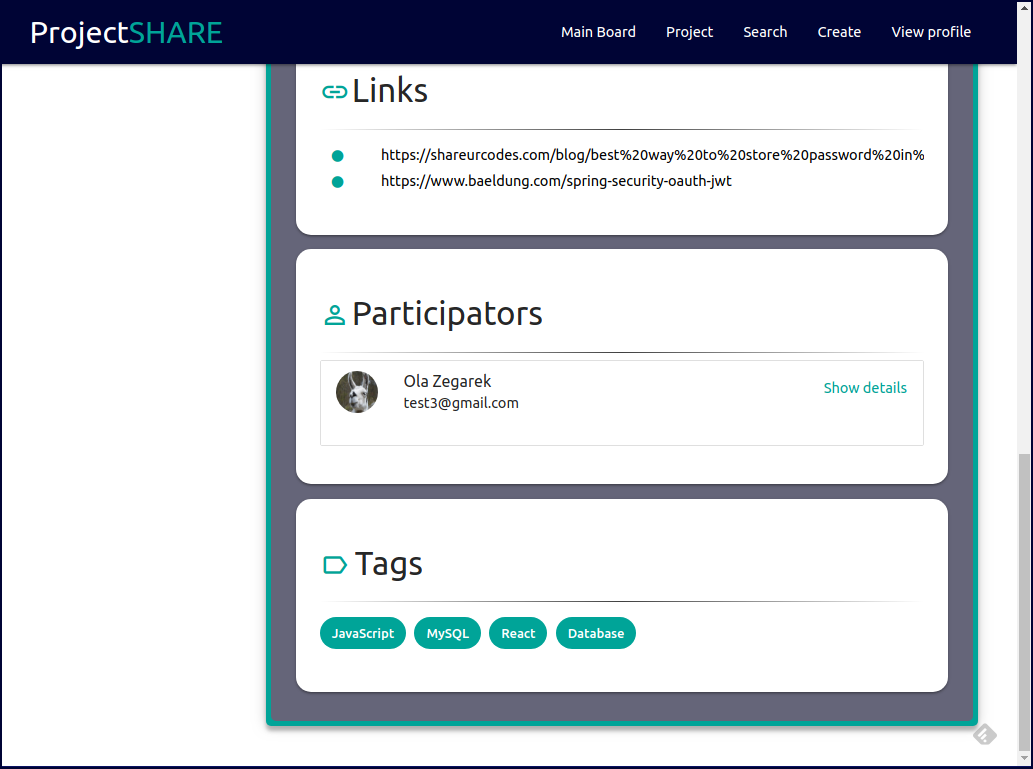
\includegraphics[scale=0.35]{screenProject2}
	}
	\caption{Widok rozszerzonego opisu projektu cz.2}
	\centering
\end{figure}

\bigskip
\bigskip
\bigskip
\bigskip
\bigskip
\bigskip
\bigskip
\bigskip
\bigskip
\bigskip
\bigskip
\bigskip
\bigskip
\bigskip
\bigskip
\bigskip

Kolejnym elementem aplikacji jest widok wyszukiwarki projektów. Podając nazwę można wyszukać podobne inicjatywy oraz przefiltrować je na podstawie tagów. Po pomyślnym wyszukaniu wyświetla się lista projektów w formacie podobnym jak przy głównym panelu.



\begin{figure}[h!]
	\makebox[\textwidth][c]{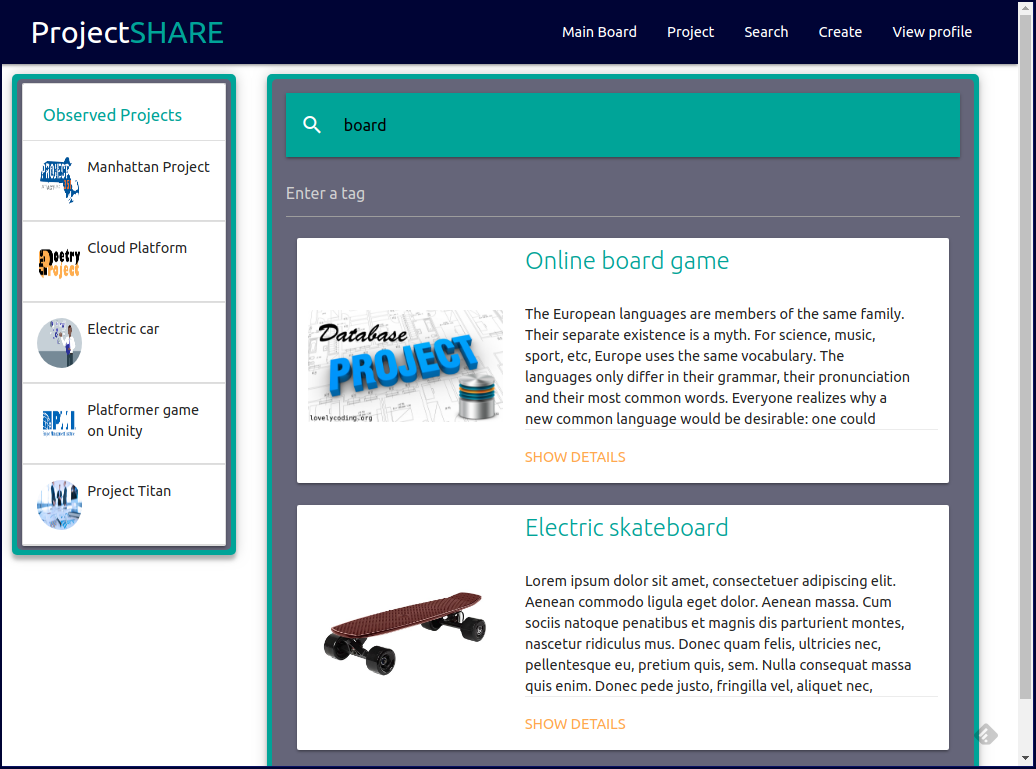
\includegraphics[scale=0.30]{screenSearch}
	}
	\caption{Widok wyszukiwarki projektów}
	\centering
\end{figure}



Do stworzenia projektu został zaprojektowany specjalny widok \textit{CreateProject}. Ułożenie poszczególnych elementów jest podobne jak przy widoku wyświetlania rozszerzonego opisu, ponieważ użytkownik może mieć wtedy wstępne wyobrażenie jaki będzie widok końcowy. Przy tworzeniu projektu należy podać jego nazwę, opis, adres URL do zdjęcia, zaznaczyć czy jest to projekt publiczny czy prywatny, uzupełnić detale, linki oraz oznaczyć go tagami. Po pomyślnym wypełnieniu formularza odblokowany zostaje przycisk \textit{Create}, a użytkownik może stworzyć projekt.

\begin{figure}[h!]
	\makebox[\textwidth][c]{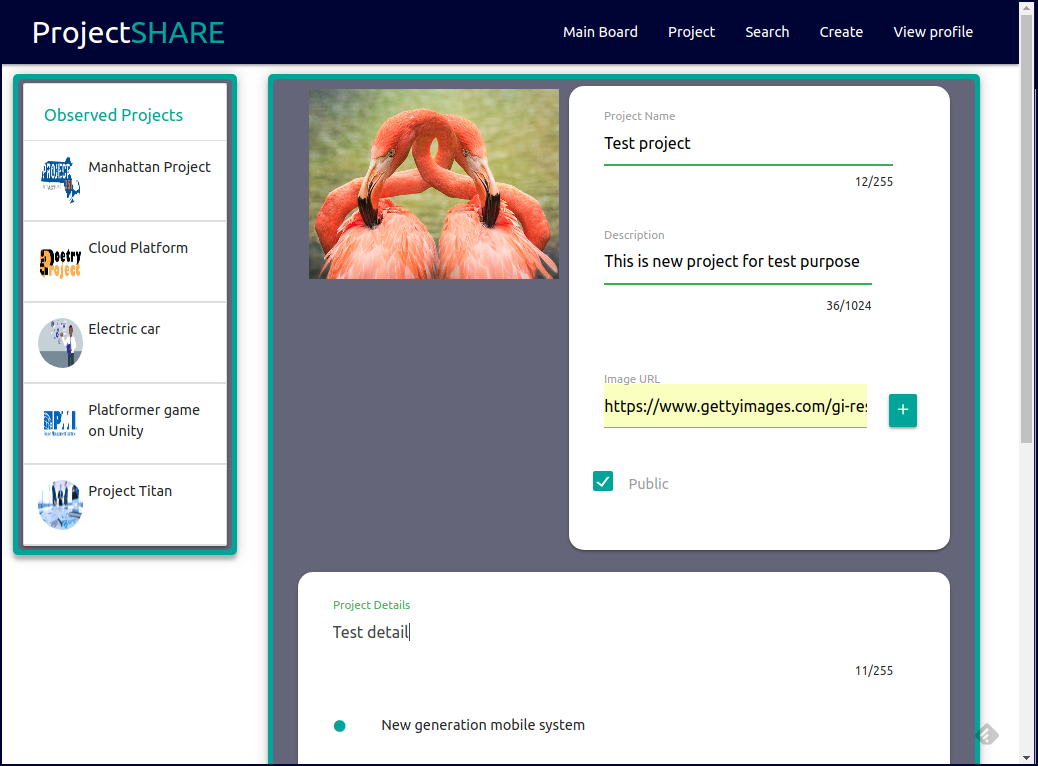
\includegraphics[scale=0.30]{screenCreate1}
	}
	\caption{Widok tworzenia projektu cz.1}
	\centering
\end{figure}

\clearpage

\begin{figure}[h!]
	\makebox[\textwidth][c]{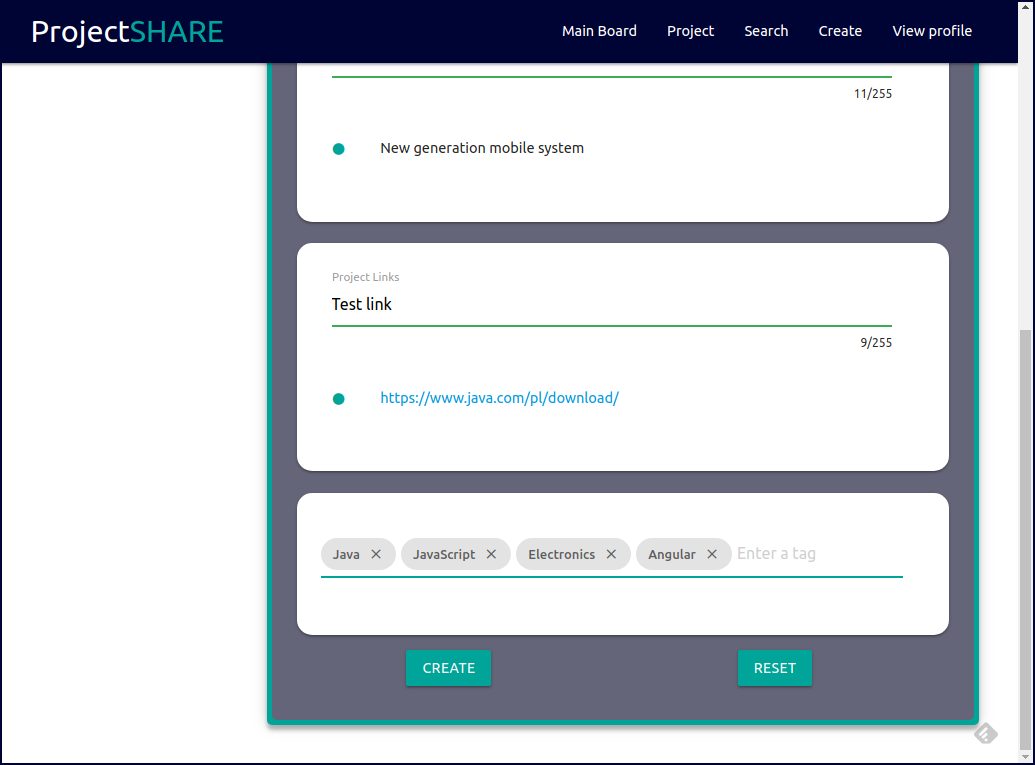
\includegraphics[scale=0.30]{screenCreate2}
	}
	\caption{Widok tworzenia projektu cz.2}
	\centering
\end{figure}


Ostatnim widokiem jest widok użytkownika. Za jego pomocą można sprawdzić z jakiego kraju pochodzi, na jaką uczelnię oraz wydział uczęszczał oraz jaką specjalizacje skończył. Dodatkowo poniżej imienia oraz nazwiska widnieje adres email pozwalający na kontakt z użytkownikiem. Zgodnie z wymaganiami klienta zmieszczono również listę projektów, w których dany użytkownik bierze udział. Ma to na celu zapewnienie możliwości sprawdzenia m.in. czy jest szansa, że będzie On posiadał interesujące informacje, czy posiada odpowiednie kompetencje w danym zakresie.

\begin{figure}[h!]
	\makebox[\textwidth][c]{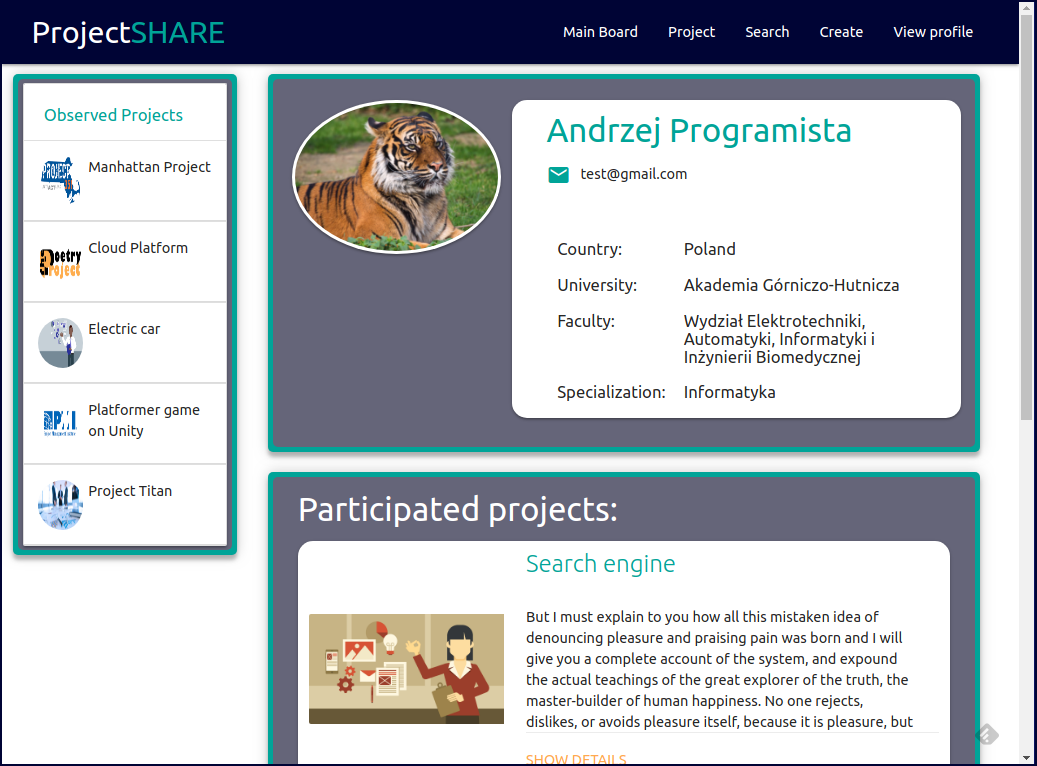
\includegraphics[scale=0.30]{screenUser}
	}
	\caption{Widok z informacjami o użytkowniku}
	\centering
\end{figure}

\clearpage

\section{Implementacja algorytmu rekomendacji}

\section{Testy systemu rekomendacji}

W celu przetestowania działania systemu rekomendacji w praktyce przygotowano specjalny zestaw danych testowych. Stworzono trzech użytkowników reprezentujących trzy osobne dziedziny zainteresowań: programowanie, mechanika, biologia. Każdy z użytkowników zaobserwował 5 projektów zgodnych z jego zainteresowaniami. Na potrzeby testu stworzono ich łącznie 30, po 10 na każdą przewidzianą dziedzinę. 
Głównym celem testu było sprawdzenie, czy na panelu projektów polecanych pojawią się projekty zgodne z zainteresowaniami danego użytkownika. Dodatkowo porównano za pomocą tabeli tagi projektów obserwowanych oraz polecanych, wraz ze współczynnikiem zgodności danego projektu z zainteresowaniami użytkownika. 


Poniżej umieszczone są wyniki przeprowadzonego testu, postaci tabel porównawczych

\begin{figure}[h!]
	\makebox[\textwidth][c]{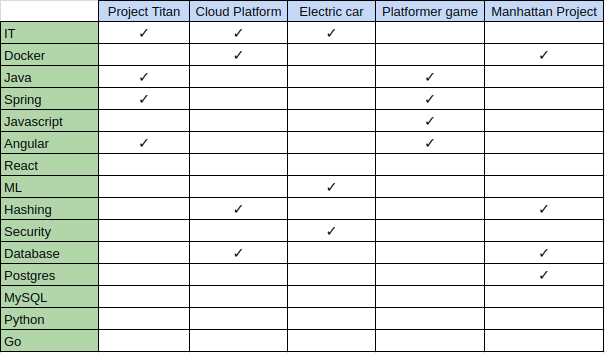
\includegraphics[scale=0.6]{tabelaprog1}
	}
	\caption{Projekty zaobserwowane przez użytkownika o zainteresowaniach programistycznych wraz z tagami}
	\centering
\end{figure}

\begin{figure}[h!]
	\makebox[\textwidth][c]{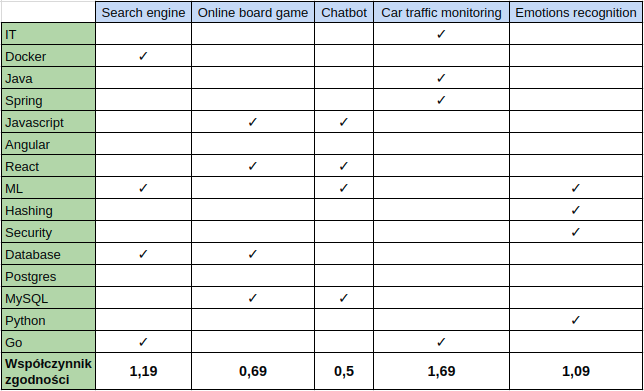
\includegraphics[scale=0.6]{tabelaprog2}
	}
	\caption{Projekty polecone użytkownikowi o zainteresowaniach programistycznych wraz z tagami oraz wyliczonym współczynnikiem zgodności}
	\centering
\end{figure}





\begin{figure}[h!]
	\makebox[\textwidth][c]{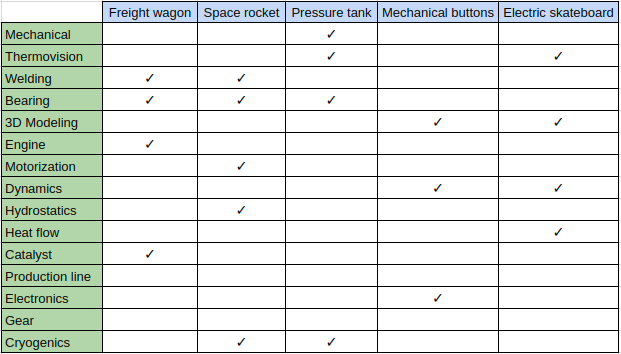
\includegraphics[scale=0.6]{tabelamech1}
	}
	\caption{Projekty zaobserwowane przez użytkownika o zainteresowaniach mechanicznych wraz z tagami}
	\centering
\end{figure}

\begin{figure}[h!]
	\makebox[\textwidth][c]{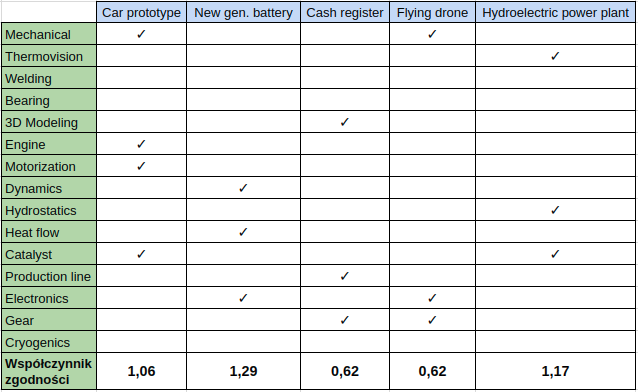
\includegraphics[scale=0.6]{tabelamech2}
	}
	\caption{Projekty polecone użytkownikowi o zainteresowaniach mechanicznych wraz z tagami oraz wyliczonym współczynnikiem zgodności}
	\centering
\end{figure}





\begin{figure}[h!]
	\makebox[\textwidth][c]{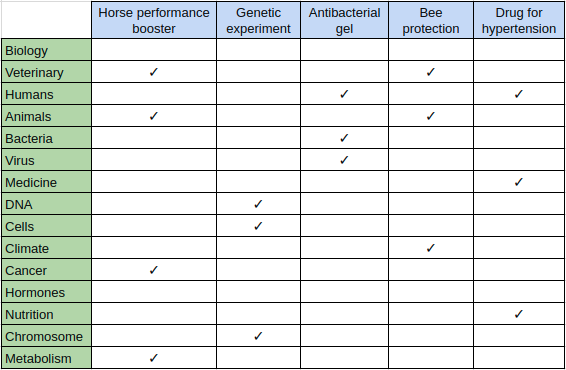
\includegraphics[scale=0.6]{tabelabiol1}
	}
	\caption{Projekty zaobserwowane przez użytkownika o zainteresowaniach biologicznych wraz z tagami}
	\centering
\end{figure}

\begin{figure}[h!]
	\makebox[\textwidth][c]{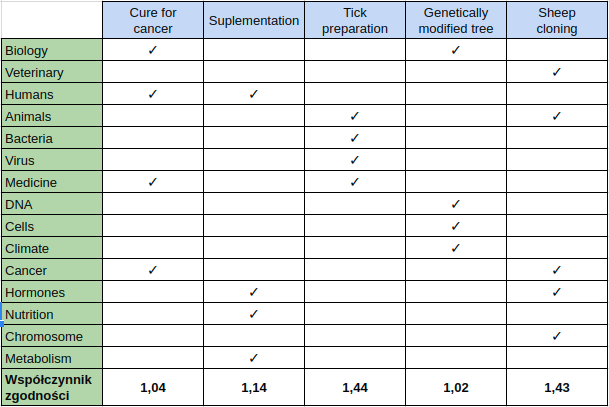
\includegraphics[scale=0.6]{tabelabiol2}
	}
	\caption{Projekty polecone użytkownikowi o zainteresowaniach biologicznych wraz z tagami oraz wyliczonym współczynnikiem zgodności}
	\centering
\end{figure}

\chapter{Podsumowanie}
Celem niniejszej pracy inżynierskiej było zaprojektowanie oraz zaimplementowanie kompletnej aplikacji, umożliwiającej komunikację oraz wymianę informacji między autorami projektów. Proces implementacji odbywał się zgodnie z metodyką zwinną oraz zastosowano w nim kilka wybranych technik wytwarzania oprogramowania stosowanych w obrębie wyżej wymienionej metodyki. Jednym z elementów aplikacji jest system rekomendacji, którego zadaniem było polecanie projektów dostosowanych do zainteresowań użytkownika. Jednocześnie miał on za zadanie filtrować projekty nie związane z branżą danego użytkownika. Do jego implementacji wykorzystano algorytm Content-based filtering dla reprezentacji binarnej. Ponadto przy projektowaniu i implementacji skupiono się na wygodnym i przejrzystym interfejsie użytkownika. Finalnie dostarczono produkt o minimalnej wartości biznesowej zgodny z ustalonymi wymaganiami.

\section{Perspektywy rozwoju}

Na implementację aplikacji został przeznaczony określony czas, w którym należało spełnić konkretne wymagania. Wymóg ten sprawił, że dostarczenie wszystkich funkcjonalności określonych przez klienta stało się niemożliwe przy obecnej zdolności. W tej sytuacji konieczne było ustalenie najważniejszych \textit{User stories}, które mogły zostać zaimplementowane w danym czasie. Za pomocą techniki \textit{Planning poker} ustalono koszt wyprodukowania każdej z nich, co pozwoliło na określenie, które z nich mają zostać wykonane. W ramach dalszego rozwoju aplikacji należałoby skupić się na dostarczeniu funkcjonalności, które nie były możliwe do spełnienia tzn. komunikator, powiadomienia email, wysyłanie zaproszeń do użytkowników. Przy ustaleniu planu na kolejną iterację należy również pamiętać o możliwości pojawienia się nowych wymagań użytkownika takich jak np. możliwość rejestrowania oraz edycji użytkowników, panel administratora. Historyjki te należy ponownie ocenić za pomocą \textit{Planning Poker} oraz ustalić wartość biznesową każdej z nich.

\section{Ocena systemu rekomendacji}

Obecna wersja zaimplementowanego systemu rekomendacji dobrze spełnia zadania określone we wstępnych wymaganiach. Pozwala on na wyświetlenie użytkownikowi tylko tych projektów, które są dla niego potencjalnie interesujące. Jednakże na tym etapie występuje kilka problemów wymagających naprawy bądź ulepszenia. Pierwszym z nich jest problem zimnego startu. Pomimo faktu, że system opiera się na zawartości przez co nie potrzebuje ogromnej ilości danych do stworzenia wystarczająco dobrej rekomendacji, wciąż pojawia się problem zimnego startu. Nowo utworzony użytkownik musi zaobserwować jakikolwiek projekt, aby rekomendacja mogła zostać stworzona. Rozwiązaniem tego problemu może być przerobienie algorytmu Content-based na algorytm hybrydowy. W przypadku, gdy użytkownik nie zaobserwowałby żadnego projektu predykcja mogłaby zostać osiągnięta za pomocą danych takich jak kraj, uczelnia, specjalizacja. Hybrydowy system rekomendacji mógłby zastosować algorytm Collaborative filtering np. do polecenia projektów osób z taką samą specjalizacją jak użytkownik docelowy. Innym problemem który występuje jest wzrost złożoności obliczeniowej proporcjonalny do ilości nowych danych. Content-based filtering tworzy predykcję na podstawie wszystkich rozpatrywanych elementów, przez co im większa ilość danych tym większa liczba obliczeń. Problem ten może zostać naprawiony poprzez odpowiednią optymalizację algorytmu, zastosowanie innych struktur danych oraz wykonanie obliczeń na chmurze obliczeniowej. Dodatkową możliwością ulepszenia działania algorytmu jest wprowadzenie oznaczenia projektów jako nie interesujące. Takie oznaczenie spowodowałoby większą różnorodność oraz lepsze dopasowanie profilu użytkownika, jednak do określenia dobrej predykcji wymagałoby większego zbioru danych.




% itd.
% \appendix
% \include{dodatekA}
% \include{dodatekB}
% itd.

\printbibliography

\end{document}
